\chapter{Conjuntos y funciones}

\section{Introducción}

Este capítulo introduce los conceptos fundamentales de \glspl{conjunto} y \glspl{funcion}, herramientas matemáticas esenciales en diversas áreas de la ingeniería. Se aborda la definición de conjunto, sus diferentes representaciones (extensión y comprensión), y las operaciones básicas entre conjuntos como unión, intersección, diferencia y complemento. Se estudian las relaciones de pertenencia e inclusión entre conjuntos, y el concepto de conjunto vacío y conjunto universal.

Además, se introduce el concepto de función, tipos de funciones (inyectiva, sobreyectiva, biyectiva) y su representación cartesiana. Se estudian operaciones entre funciones como la composición y la función inversa, y se analizan ejemplos de funciones especiales relevantes en matemáticas.


\subsection{Relevancia en ingeniería}

\begin{itemize}
	\item \textit{Modelado de sistemas}: Los conjuntos se utilizan para representar colecciones de objetos o elementos en un sistema, como por ejemplo, un conjunto de usuarios de una red de telecomunicaciones, un conjunto de componentes en un circuito eléctrico o para analizar las propiedades del suelo de un terreno;
	\item \textit{Análisis de datos}: Las funciones son esenciales para modelar relaciones entre variables en el análisis de datos, como la resistencia de un material en función del tiempo o modelación de fenómenos espaciales, como la altitud de un terreno.
	\item \textit{Programación}: Los conceptos de conjuntos y funciones son fundamentales en la programación, donde se utilizan para definir estructuras de datos y algoritmos.
	\item \textit{Optimización}: Las funciones se utilizan en problemas de optimización para representar la función objetivo que se busca maximizar o minimizar.
\end{itemize}

\section{Conjuntos} \label{sec:conjuntos}

\index{conjunto}

\subsection{Definición intuitiva de conjunto}
\vspace{1em}
\begin{fmd-definition}[Conjunto]
	Un \gls{conjunto} es una colección o agrupación de objetos, llamados \glspl{elemento} que comparten una característica común.
\end{fmd-definition}

Estos objetos pueden ser números, letras, personas, animales, o cualquier otra cosa que deseemos considerar juntos. En otras palabras, un conjunto es como una ``caja'' que contiene elementos relacionados.

\begin{fmd-example}[Conjuntos]
	\begin{enumerate}
		\item Conjunto de números naturales ($\N$):
		
		El conjunto de todos los números naturales es un ejemplo fundamental. Se denota como $\N$ y contiene los números $\{ 1, 2, 3, 4, 5, \ldots \}$.
		
		\item Conjunto de vocales: $\{a, e, i, o, u\}$.
		
		\item Conjunto de días de la semana:
		
		$\{ \text{lunes}, \text{martes}, \text{miércoles}, \text{jueves}, \text{viernes}, \text{sábado}, \text{domingo} \}$
		
		\item Conjunto de números pares: $\{2, 4, 6, 8, 10, \ldots \}$
		
		\item Conjunto de colores primarios: $\{\text{rojo}, \text{azul}, \text{amarillo}\}$.
	\end{enumerate}
\end{fmd-example}

\begin{lgnote}
	En un conjunto, los elementos no se repiten, y el orden no importa. Los elementos de un conjunto se escriben entre llaves $\{ \}$.
\end{lgnote}

\subsubsection{Notación}
Para denotar conjuntos utilizaremos generalmente letras mayúsculas $(A, B, C, \ldots)$, y para especificar elementos se usarán letras minúsculas \( (a, b, c, \ldots) \), a menos que dichos elementos sean, a su vez, conjuntos.

\subsubsection{Conjuntos numéricos}

Las notaciones usuales para caracterizar conjuntos numéricos son las siguientes:

\begin{itemize}
	\item $\N$: conjunto de números naturales;
	\item $\Z$: conjunto de números enteros;
	\item $\Q$: conjunto de números racionales;
	\item $\R$: conjunto de números reales;
	\item $\C$: conjunto de números complejos;
\end{itemize}

\subsubsection{Conjuntos especiales}

\begin{itemize}
	\item El \gls{conjuntouniversal}, \index{conjunto!universal} denotado como \glsentrysymbol{conjuntouniversal}, es el que contiene todos los elementos posibles que estamos considerando en un contexto particular. Es el conjunto más grande en ese contexto y actúa como un marco de referencia para otros conjuntos más pequeños.
	
	Por ejemplo, si estamos trabajando con números naturales, el conjunto universal sería \(\mathbb{N}\), que incluye todos los números positivos enteros: \(\{1, 2, 3, 4, \ldots\} \).
	
	\item El \gls{conjuntovacio}, \index{conjunto!vacío}  denotado como \glsentrysymbol{conjuntovacio}, es aquel que no contiene ningún elemento. El conjunto vacío es único, en otras palabras, todos los conjuntos vacíos son iguales.
	
	Por ejemplo, el conjunto vacío puede representar el conjunto de números reales que son mayores que 10 y menores que 5. Dado que no hay números que cumplan esta condición, el conjunto resultante es vacío: \glsentrysymbol{conjuntovacio}.
	
	\item Un \gls{conjuntounitario} está formado por un único elemento. Ejemplo $A = \{ a \}$.
\end{itemize}

\subsection{Relaciones de pertenencia e inclusión}

\subsubsection{Relación de pertenencia}

Para indicar la \gls{pertenencia} \index{pertenencia} de un elemento a un conjunto será utilizado el símbolo \glsentrysymbol{pertenencia}.

La proposición $a \in A$ se lee ``$a$ \textit{pertenece} a $A$'', o bien ``el elemento $a$ \textit{pertenece} al conjunto $A$''. Su negación es $a \not \in A$, que se lee ``$a$ \textit{no pertenece} a $A$''

\subsubsection{Notación por extensión}

La \gls{notacionextension} \index{conjunto!extensión} lista cada elemento del conjunto de forma individual.

\begin{fmd-example}[Notación por extensión]
	\begin{enumerate}
		\item Conjunto de números pares menores que 10: $E = \{2, 4, 6, 8\}$
		\item Conjunto de vocales: \(V = \{a, e, i, o, u\}\)
		\item Conjunto de meses del año: \(M = \{\text{enero}, \text{febrero}, \ldots, \text{diciembre}\}\)
	\end{enumerate}
\end{fmd-example}

\subsubsection{Notación por comprensión}
\index{conjunto!comprensión}
En la \gls{notacioncompresion}, describimos las propiedades o características que deben cumplir los elementos del conjunto, luego, utilizamos una condición lógica para definir el conjunto.

En general su estructura tiene la forma:
\[ A = \{ x \in U \mid P(x) \}\]
el conjunto cuyos elementos verifican la propiedad $P(x)$, o más brevemente, si $U$ está sobreentendido:
\[ A = \{ x \mid P(x) \}\]
se lee: ``$A$ es el conjunto formado por los elementos $x$, tales que $P(x)$'', en donde $P(x)$ es un función proposicional.

Un objeto $a$ del universal pertenece al conjunto $A$ \gls{siysolosi} verifica la propiedad $P(x)$, en consecuencia, el elemento $a$ no pertenece al conjunto $A$ si no cumple la propiedad $P(x)$.

\begin{fmd-example}[Notación por comprensión]
	\begin{enumerate}
		\item Conjunto de números pares: \(P = \{x \in \mathbb{N} \mid x = 2 k \mbox{ con } k \in \mathbb{N} \}\)
		
		``Son todos los números naturales $x$ tal que cada $x$ es igual al doble de un número natural $k$''.
		
		\item Conjunto de números primos menores que 20: \[N = \{x \in \mathbb{N} \mid (x \mbox{ es un número primo}) \mbox{ y } (x < 20) \}\]
		``Son todos los números naturales que son a la vez primos y menores que 20''
		
		\item Conjunto de letras del alfabeto: \(L = \{x \mid x \mbox{ es una letra del alfabeto}\}\)
		
		``El conjunto de elementos $x$ tal que $x$ es una letra del alfabeto''
		
		\item El \gls{conjuntovacio} puede definirse simbólicamente como: $\emptyset = \{ x \mid x \ne x \}$
		
		``Los elementos $x$ tal que cada $x$ es distinto de sí mismo'' (no existen tales elementos).
		
		En este caso la propiedad relativa a $x$ es $P(x): x \ne x$, la cual resulta falsa cualquiera sea $x$.
		
		\item Si $A$ es un conjunto unitario cuyo único elemento es $a$, escribiremos:
		\[ A = \{ a\} = \{ x \mid x = a \} \]
	\end{enumerate}
\end{fmd-example}

\subsubsection{Inclusión}
La \gls{inclusion} tiene la siguiente definición: \index{inclusión}

\begin{fmd-definition}[Inclusión]
	Sean $A$ y $B$ dos conjuntos, si ocurre que todo elemento de $A$ pertenece a $B$, diremos que $A$ está incluido en $B$, o que $A$ es parte de $B$, o que $A$ es un subconjunto de $B$.
	
	Notación:  \[A \subset B\]
\end{fmd-definition}

\begin{fmd-example}[Inclusión]
	\begin{enumerate}
		\item Consideremos los conjuntos: \(A = \{1, 2\}\) y \(B = \{1, 2, 3\}\).
		
		En este caso, \(A \subset B\), ya que todos los elementos de \(A\) (1 y 2) también pertenecen a \(B\).
		
		\item Consideremos los conjuntos:
		
		\begin{itemize}
			\item \(C = \{x \mid x \mbox{ es un número par}\}\)
			\item \(D = \{x \mid x \mbox{ es un número entero}\}\)
			
			Aquí, \(C \subset D\), ya que todo número par es también entero.
		\end{itemize}
	\end{enumerate}
\end{fmd-example}


\begin{itemize}
	\item Propiedades de la inclusión
	\begin{enumerate}[label=\roman*)]
		\item \textbf{Reflexibidad}: Todo conjunto es parte de sí mismo.
		\[ A \subset A \]
		\item \textbf{Transitividad}: Si un conjunto es parte de otro y este es parte de un tercero, el primero está incluido en el tercero:
		\[\mbox{Si } A \subset B \mbox{ y } B \subset C \mbox{ entonces } A \subset C \]
		\item \textbf{Antisimetría}: Si un conjunto es parte de otro y éste es parte del primero, entonces son iguales\footnote{Este hecho se usa para establecer la igualdad de conjuntos dada en la definición \ref{def:igualdad_conjuntos}}.
		\[\mbox{Si } A \subset B \mbox{ y } B \subset A \mbox{ entonces } A = B \]
	\end{enumerate}
	
	\item Observaciones:
	
	\begin{enumerate}
		\item En repetidas ocasiones se necesitará demostrar que un conjunto es parte de otro; entonces, de acuerdo con la definición, será suficiente demostrar que cualquier elemento del primero pertenece al segundo, esto significa que en la inclusión no puede darse que haya un elemento de $A$ que no pertenezca a $B$.
		\[A \subset B \mbox{ significa que, si } x \in A \mbox{ también } x \in B \]
		
		\item El conjunto vacío es subconjunto de cualquier conjunto.
		\[ \emptyset \subset A \]
	\end{enumerate}
\end{itemize}

\subsubsection{Igualdad de conjuntos}
\vspace{1em}
\index{conjuntos!igualdad}
\begin{fmd-definition}[Igualdad de conjuntos] \label{def:igualdad_conjuntos}
	Dos conjuntos $A$ y $B$ son iguales, es decir, se cumple la \gls{igualdad_conjuntos} $A = B$, si y solo si todo elemento de $A$ pertenece a $B$ y todo elemento de $B$ pertenece a $A$, en otras palabras, dos conjuntos son iguales si se contienen mutuamente.
	\[A = B \mbox{ si y sólo si } A \subset B \mbox{ y } B \subset A \]
\end{fmd-definition}

\subsubsection{Diagrama de Venn}
\index{diagrama Venn}

El \gls{venn} es una representación visual de los conjuntos utilizando diagramas llamados de Venn en homenaje a su autor\footnote{John Venn (1834-1923), matemático y lógico británico.}. En este sentido, el conjunto universal suele representarse por un rectángulo y los conjuntos por recintos cerrados. Es claro que todo elemento de $A$ pertenece a $U$, o sea, $A \subset U$. $A$, $B$ y $C$ subconjuntos de $U$, como indica el diagrama de la fig. \ref{fig:Venn}.

\begin{figure}[H]
	\centering
	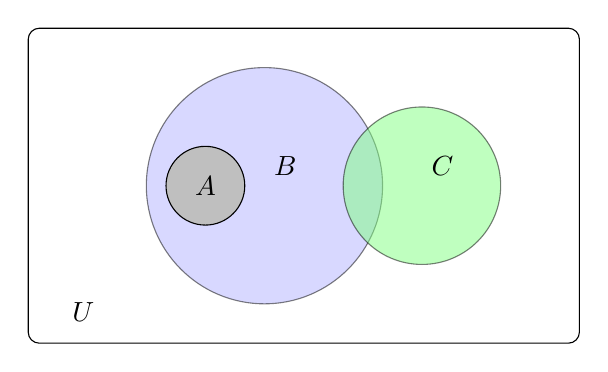
\begin{tikzpicture}
		% Conjunto Universal U
		\draw[rounded corners] (-3,-2) rectangle (4,2) node[pos=.1] {$U$};
		
		% Conjunto B
		\draw[fill=blue!30, opacity=.5] (0,0) circle (1.5cm) node[opacity=1, above right] {$B$};
		
		% Conjunto C
		\draw[fill=green!50, opacity=.5] (2,0) circle (1cm) node[opacity=1, above right] {$C$};
		
		% Conjunto A
		\draw[fill=gray!50] (-.75, 0) circle (0.5cm) node {$A$};
	\end{tikzpicture}
	\caption{Diagrama de Venn}
	\label{fig:Venn}
\end{figure}

\subsection{Operaciones con conjuntos}

\subsubsection{Unión \glsentrysymbol{union}}
\vspace{1em} \index{unión}
\begin{fmd-definition}[Unión]
	La \gls{union} de dos conjuntos \(A\) y \(B\) consiste en todos los elementos que pertenecen a \(A\), a \(B\), o a ambos conjuntos.
	
	Notación: \(A \cup B\)
	
	Formalmente:
	\[ A \cup B = \left\{ x \mid x \in A \mbox{ o } x \in B \right\} \]
\end{fmd-definition}

\begin{itemize}
	\item Diagrama de Venn
	\begin{figure}[H]
		\centering
		\begin{venndiagram2sets}
			\fillA \fillB
		\end{venndiagram2sets}
		\caption*{$A \cup B$}
	\end{figure}
	
	\item Propiedades:
	\begin{enumerate}[label=\roman*)]
		\item Idempotencia\footnote{La idempotencia se define en la pág. \index{idempotencia} \pageref{def:idempotencia}, definición \ref{def:idempotencia}.}: \( A \cup A = A \)
		\item Asociatividad: \( \left( A \cup B \right) \cup C = A \cup \left( B \cup C \right) \)
		\item Conmutatividad: \( A \cup B = B \cup A\)
	\end{enumerate}
\end{itemize}

\begin{example}[Unión]
	Si \(A = \{1, 2, 3\}\) y \(B = \{3, 4, 5\}\), entonces \(A \cup B = \{1, 2, 3, 4, 5\}\).
\end{example}

\subsubsection{Intersección \glsentrysymbol{interseccion}}
\vspace{1em} \index{intersección}
\begin{fmd-definition}[Intersección]
	La \gls{interseccion} de dos conjuntos \(A\) y \(B\) contiene los elementos que pertenecen tanto a \(A\) como a \(B\).
	
	Notación: \(A \cap B\)
	
	Formalmente:
	\[ A \cap B = \left\{ x \mid x \in A \mbox{ y } x \in B \right\} \]
\end{fmd-definition}

\begin{itemize}
	\item Diagrama de Venn
	\begin{figure}[H]
		\centering
		\begin{venndiagram2sets}
			\fillACapB
		\end{venndiagram2sets}
		\caption*{\(A \cap B \)}
	\end{figure}
	
	\item Propiedades:
	\begin{enumerate}[label=\roman*)]
		\item Idempotencia: \( A \cap A = A \) \index{idempotencia}
		\item Asociatividad: \( \left( A \cap B \right) \cap C = A \cap \left( B \cap C \right) \) \index{asociatividad}
		\item Conmutatividad: \( A \cap B = B \cap A\) \index{conmutatividad}
	\end{enumerate}
\end{itemize}

\begin{example}[Intersección]
	Si \(A = \{1, 2, 3\}\) y \(B = \{3, 4, 5\}\), entonces \(A \cap B = \{3\}\).
\end{example}

\subsubsection{Complemento $(A^c)$}
\vspace{1em} \index{complemento}

\begin{fmd-definition}[Complemento]
	El \gls{complemento} de un conjunto \(A\) con respecto a un conjunto universal \(U\) contiene todos los elementos que no están en \(A\).
	Notación: \(A^c\) o \(\overline{A}\) o \(A'\)
	
	Formalmente:
	\[ A^c = \left\{ x \mid x \in U \mbox{ y } x \not \in A \right\} \]
\end{fmd-definition}

\begin{itemize}
	\item Diagrama de Venn
	
	\begin{figure}[H]
		\centering
		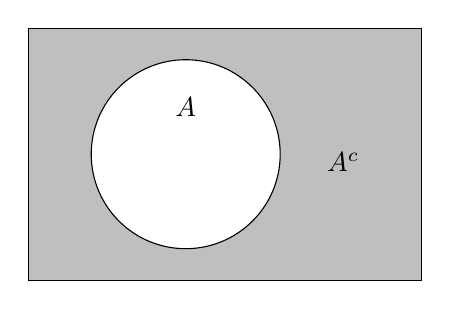
\begin{tikzpicture}[scale=1]
			\filldraw[fill=lightgray] (0, 0) rectangle (5,3.2); % Rectángulo del universo
			\filldraw[fill=white] (2, 1.6) circle (1.2); % Dibuja y rellena el conjunto A
			
			\node at (2, 2.2) {$A$}; % Etiqueta el conjunto A
			\node at (4, 1.5) {$A^c$}; % Etiqueta el complemento de A
		\end{tikzpicture}
		\caption*{\(A^c\)}
	\end{figure}
	\item Propiedades:
	\begin{enumerate}
		\item Involución $(A^c)^c = A$.
		
		De donde: Si \( A^c = B \) entonces \( B^c = A \)
		\item $A \subset B \implies B^c \subset A^c$
		\item El complemento del vacío es el universal: \( \emptyset^c = U \)
		\item El complemento del universal es el vacío: \( U^c = \emptyset \)
	\end{enumerate}
\end{itemize}

\begin{example}[Complemento]
	Si \(U\) es el conjunto de números naturales y \(A\) el conjunto de números pares,  \(A = \{2, 4, 6, \ldots \}\), entonces \(A^c\) es el conjunto de números impares, \(A^c = \{1, 3, 5, 7, \ldots\}\).
\end{example}

\subsubsection{Diferencia $(-, \setminus)$}

\vspace{1em}
\index{conjunto!diferencia}
\begin{fmd-definition}[Diferencia de conjuntos]
	La diferencia entre dos conjuntos \(A\) y \(B\) contiene los elementos que están en \(A\) pero no en \(B\).
	
	Notación: \(A - B\) o \( A \setminus B \)
	
	Formalmente:
	\[ A \setminus B = \left\{ x \mid x \in A \mbox{ y } x \not \in B \right\} \]
\end{fmd-definition}

\begin{itemize}
	\item Diagrama de Venn
	\begin{figure}[H]
		\centering
		\begin{venndiagram2sets}
			\fillOnlyA
		\end{venndiagram2sets}
		\caption*{$A \setminus B$}
	\end{figure}
	\item Propiedades:
	\begin{enumerate}[label=\roman*)]
		\item La diferencia entre dos conjuntos es igual a la intersección del primero con el complemento del segundo: \( A \setminus B = A \cap B^c \)
	\end{enumerate}
\end{itemize}

\begin{example}[Diferencia de conjuntos]
	Si \(A = \{1, 2, 3\}\) y \(B = \{3, 4, 5\}\), entonces \(A - B = \{1, 2\}\).
\end{example}

\subsubsection{Diferencia simétrica $\triangle$}
\vspace{1em}
\index{conjunto!dif. sim.}
\begin{fmd-definition}[Diferencia simétrica]
	La \gls{difsimetrica} de dos conjuntos \(A\) y \(B\), es el conjunto que contiene los elementos que pertenecen a \(A\) o a \(B\), pero no a ambos.
	
	Notación: \(A \triangle B\)
	
	Formalmente:
	$$A \triangle B = (A \setminus B) \cup (B \setminus A)$$
	
	La diferencia simétrica es el conjunto de elementos que están en uno de los conjuntos, pero no en ambos. Es como si ``excluyéramos'' la intersección de los dos conjuntos, por lo tanto también podemos escribir:
	\[ A \triangle B = \left( A \cup B \right) \setminus \left( A \cap B \right) \]
\end{fmd-definition}

\begin{itemize}
	\item Diagrama de Venn
		\begin{figure}[H]
			\centering
			\begin{venndiagram2sets}
				\fillOnlyA \fillOnlyB
			\end{venndiagram2sets}
			\caption*{$A \triangle B$}
		\end{figure}
	
	\item Propiedades:
	\begin{enumerate}[label=\roman*)]
		\item Conmutatividad: \(A \triangle B = B \triangle A\)
		\item Asociatividad: \((A \triangle B) \triangle C = A \triangle (B \triangle C)\)
		\item Existencia del neutro\footnote{El elemento neutro se define formalmente en \ref{sec:axiomas-grupo}, pág. \pageref{sec:axiomas-grupo}}: \( A \triangle \emptyset = \emptyset \triangle A = A \)
		\item Existencia de inversas\footnote{Ibid.}: \( A \triangle A = \emptyset \)
	\end{enumerate}
\end{itemize}

\begin{example}[Diferencia simétrica]
	\
	\begin{enumerate}
		\item Consideremos los conjuntos: \(A = \{1, 2, 3, 4\}\) y \(B = \{3, 4, 5, 6\}\). Entonces, la diferencia simétrica es:
		
		$$A \triangle B = \{1, 2, 5, 6\}$$
		
		Los elementos 1 y 2 están solo en \(A\), 5 y 6 están solo en \(B\). Los elementos 3 y 4 se excluyen porque están en ambos conjuntos.
		
		\item Consideremos los conjuntos:
		\begin{itemize}
			\item \(C = \{x \mid x \mbox{ es un número par}\}\)
			\item \(D = \{x \mid x \mbox{ es un número primo}\}\)
		\end{itemize}
		
		La diferencia simétrica es:
		$$C \triangle D = \{x \mid x \text{ es par y no es 2, o } x \text{ es primo y no es 2}\}$$
		El número 2 se excluye porque es el único par que también es primo.
	\end{enumerate}
\end{example}


\subsubsection{Conjunto potencia o conjunto de partes $\mathcal{P}(A)$}
\vspace{1em}
\index{conjunto!potencia} \index{conjunto!de partes}
\begin{fmd-definition}[Conjunto potencia]
	Dado un conjunto \(A\), el \gls{conjuntopotencia} o conjunto de partes de \(A\), denotado por \glsentrysymbol{conjuntopotencia} o \(2^A\), es el conjunto de todos los subconjuntos de \(A\). 
	
	Formalmente:
	$$\mathcal{P}(A) = \{B \mid B \subseteq A\}$$
	
	El conjunto potencia de un conjunto \(A\) es una colección que contiene a todos los posibles subconjuntos de \(A\), incluyendo el conjunto vacío (\(\emptyset\)) y el propio conjunto \(A\).
\end{fmd-definition}


\begin{example}[Conjunto potencia]
	\
	\begin{enumerate}
		\item Consideremos el conjunto: \(A = \{1, 2\}\)
		
		Entonces, el conjunto potencia es:
		$$\mathcal{P}(A) = \{\emptyset, \{1\}, \{2\}, \{1, 2\}\}$$
		
		Observe que hay \(2^2 = 4\) elementos en el conjunto potencia, ya que cada elemento de \(A\) tiene dos opciones: estar o no estar en un subconjunto particular.
		
		\item Consideremos el conjunto: \(B = \{a, b, c\}\)
		
		El conjunto potencia es:
		$$\mathcal{P}(B) = \{\emptyset, \{a\}, \{b\}, \{c\}, \{a, b\}, \{a, c\}, \{b, c\}, \{a, b, c\}\}$$
		En este caso, hay \(2^3 = 8\) elementos en el conjunto potencia.
	\end{enumerate}
\end{example}

\begin{lgnote}
	En general, si un conjunto \(A\) tiene \(n\) elementos, entonces su conjunto potencia \(\mathcal{P}(A)\) tiene \(2^n\) elementos.
\end{lgnote}

\subsubsection{Producto cartesiano}
\vspace{1em}
\index{producto!cartesiano}
\begin{fmd-definition}[Producto cartesiano]
	El \gls{productocartesiano} de dos conjuntos \(A\) y \(B\), es el conjunto de todos los pares ordenados \((a, b)\) donde el primer elemento \(a\) pertenece al conjunto \(A\) y el segundo elemento \(b\) pertenece al conjunto \(B\).

	Notación: \(A \times B\)
	
	Formalmente:
	$$A \times B = \{(a, b) \mid a \in A \text{ y } b \in B\}$$
	
	Esto es, el producto cartesiano combina cada elemento de un conjunto con cada elemento del otro conjunto, formando pares ordenados donde el orden de los elementos es importante.
\end{fmd-definition}


\begin{example}[Producto cartesiano]
	\
	\begin{enumerate}
		\item Consideremos los conjuntos: \(A = \{1, 2\}\) y \(B = \{x, y\}\), entonces, el producto cartesiano es:
		$$A \times B = \{(1, x), (1, y), (2, x), (2, y)\}$$
		
		\item Consideremos los conjuntos: \(C = \{a, b\}\) y \(D = \{1, 2, 3\}\), el producto cartesiano es:
		$$C \times D = \{(a, 1), (a, 2), (a, 3), (b, 1), (b, 2), (b, 3)\}$$
	\end{enumerate}
\end{example}

\begin{itemize}
	\item Observaciones:
	
	\begin{enumerate}
		\item El producto cartesiano no es conmutativo, en general, \(A \times B \neq B \times A\).
		\item Si \(A\) tiene \(m\) elementos y \(B\) tiene \(n\) elementos, entonces \(A \times B\) tiene \(m \cdot n\) elementos.
		\item El producto cartesiano se puede extender a más de dos conjuntos. Por ejemplo, el producto cartesiano de tres conjuntos \(A\), \(B\) y \(C\) es:
		$$A \times B \times C = \{(a, b, c) \mid a \in A, b \in B, c \in C\}$$
		\item Si los elementos son del mismo conjunto $A$:
		\[ A \times A \times A = A^3 = \{(a, b, c) \mid a, b, c \in A\} \]
	\end{enumerate}
	
	\item Propiedades:
	\begin{enumerate}[label=\roman*)]
		\item El producto cartesiano es \textbf{distributivo} respecto de la unión:
		\[ \left( A \cup B \right) \times C = \left( A \times C \right) \cup \left( B \times C \right) \]
	\end{enumerate}
	
\end{itemize}


\subsection{Álgebra de conjuntos} \label{sec:algebra_conjuntos}
\index{álgebra!conjuntos}
\subsubsection{Propiedades fundamentales}

\begin{itemize}
	\item \textbf{Idempotencia}:
	\begin{itemize}[itemsep=0pt]
		\item \( A \cup A = A \)
		\item \( A \cap A = A \)
	\end{itemize}
	\item \textbf{Conmutatividad}:
	\begin{itemize}[itemsep=0pt]
		\item \(A \cup B = B \cup A\)
		\item \(A \cap B = B \cap A\)
	\end{itemize}
	
	\item \textbf{Asociatividad}:
	\begin{itemize}[itemsep=0pt]
		\item \((A \cup B) \cup C = A \cup (B \cup C)\)
		\item \((A \cap B) \cap C = A \cap (B \cap C)\)
	\end{itemize}
	
	\item \textbf{Distributividad}:
	\begin{itemize}[itemsep=0pt]
		\item \(A \cup (B \cap C) = (A \cup B) \cap (A \cup C)\)
		\item \(A \cap (B \cup C) = (A \cap B) \cup (A \cap C)\)
	\end{itemize}
		
	\item \textbf{Leyes de De Morgan}:
	
	\begin{enumerate}[label={\textbf{\arabic*})}]
		\item El complemento de la unión de dos conjuntos es igual a la intersección de los complementos de dichos conjuntos.
		\[ (A \cup B)^c = A^c \cap B^c \]
		
		\item El complemento de la intersección de dos conjuntos es igual a la unión de los complementos de dichos conjuntos.
		\[ (A \cap B)^c = A^c \cup B^c \]
	\end{enumerate}
	
	\item\textbf{Elemento neutro}\footnote{El concepto de elemento neutro se presenta en detalle en la sección \ref{sec:axiomas-grupo}, pág. \pageref{sec:axiomas-grupo}}:
	\begin{itemize}
		\item De la unión es el conjunto vacío: \(A \cup \emptyset = A\)
		\item De la intersección es el universal: \(A \cap U = A\)
		\item De la diferencia simétrica es el conjunto vacío: \( A \triangle \emptyset = \emptyset \triangle A = A \)
	\end{itemize}
	
	\item \textbf{Existencia de inversas\footnote{ibid.}}:
	\begin{itemize}
		\item Para la diferencia simétrica, $A$ es su propia inversa: \( A \triangle A = \emptyset \)
	\end{itemize}
	
	\item \textbf{Otras propiedades}:
	\begin{itemize}
		\item \(A \cup A^c = U\)
		\item \(A \cap A^c = \emptyset\)
	\end{itemize}
	
\end{itemize}

\subsubsection{Operaciones generalizadas}

\begin{itemize}
	\item \textbf{Unión generalizada} \index{unión!generalizada}
	
	Dada una colección finita de conjuntos \( \{ A_1, A_2, \dots, A_n \} \) la unión generalizada de estos conjuntos se denota por:
	\[ A_1 \cup A_2 \cup \dots \cup A_n = \bigcup_{i=1}^n A_i  \]
	Se define como el conjunto que contiene todos los elementos que pertenecen a \textit{al menos uno} de los conjuntos \(A_i\).
	
	Formalmente:
	
	Si definimos el conjunto de índices \( I_n = \{ 1, 2, \dots, n \} \) (conjunto de los $n$ primeros números naturales):
	\[ \bigcup_{i=1}^n A_i = \left\{ x \ | \ x \in A_i \mbox{ para algún } i \in I_n \right\} \]
	
	Si el conjunto $I_n$ se identifica con $\N$ (conjunto de números naturales):
	\[ \bigcup_{i=1}^\infty A_i = \left\{ x \ | \ x \in A_i \mbox{ para algún } i \in \N \right\} \]
	
	\item \textbf{Intersección generalizada} \index{intersección!generalizada}
	
	Dada una colección finita de conjuntos \( \{ A_1, A_2, \dots, A_n \} \) la intersección generalizada de estos conjuntos se denota por:
	\[ A_1 \cap A_2 \cap \dots \cap A_n = \bigcap_{i=1}^n A_i  \]
	Se define como el conjunto que contiene todos los elementos que pertenecen a \textit{todos} los conjuntos \(A_i\).
	
	Formalmente:
	\[ \bigcap_{i=1}^n A_i = \left\{ x \ | \ x \in A_i \ \forall i \in I_n \right\} \]
	
	Si el conjunto $I_n$ se identifica con $\N$:
	\[ \bigcap_{i=1}^\infty A_i = \left\{ x \ | \ x \in A_i \ \forall i \in \N \right\} \]
	
	\item \textbf{Leyes de De Morgan generalizadas}
	
	\begin{enumerate}
		\item El complemento de la unión es igual a la intersección de los complementos. 
		\[ \left( \bigcup_{i \in I} A_i \right)^c = \bigcap_{i\in I} A_i^c \]
		\item El complemento de la intersección es igual a la unión de los complementos.
		\[ \left( \bigcap_{i \in I} A_i \right)^c = \bigcup_{i\in I} A_i^c \]
	\end{enumerate}
\end{itemize}

\begin{fmd-example}[Unión e intersección generalizadas]
	Consideremos los conjuntos:
	\begin{itemize}[itemsep=0pt]
		\item \(A_1 = \{1, 2, 3\}\)
		\item \(A_2 = \{2, 3, 4\}\)
		\item \(A_3 = \{3, 4, 5\}\)
	\end{itemize}
	Entonces:
	\[\bigcup_{i=1}^{3} A_i = \{1, 2, 3, 4, 5\}\]
	\[\bigcap_{i=1}^{3} A_i = \{3\}\]
\end{fmd-example}

\subsubsection{Uniones disjuntas}
\vspace{1em}
\index{unión!disjunta}
\begin{fmd-definition}[Uniones disjuntas]
	Se dice que una colección de conjuntos tiene \glspl{uniondisjunta} si los conjuntos son mutuamente excluyentes, es decir, si la intersección de cualquier par de conjuntos de la colección es el conjunto vacío.
	
	Formalmente, una colección de conjuntos \(\{A_i\}_{i \in I}\) es una colección de uniones disjuntas si:
	\[A_i \cap A_j = \emptyset \quad \forall i, j \in I \mbox{ con } i \neq j\]
	
	Los conjuntos en una unión disjunta no comparten ningún elemento\footnote{La noción de uniones disjuntas se puede generalizar a un número infinito de conjuntos.}.
	
	Notación:
	
	Para dos conjuntos disjuntos $A$ y $B$, es usual escribir:
	\[ A + B \]
	en lugar de $A \cup B$ para el caso $A \cap B = \emptyset$.
\end{fmd-definition}

Algunas aplicaciones:

\begin{enumerate}
	\item \textit{Partición de un conjunto}\footnote{Las particiones se estudian en la sección \ref{sec:particiones}, pág. \pageref{sec:particiones}}: Una partición de un conjunto \(A\) es una colección de subconjuntos no vacíos de \(A\) que son disjuntos dos a dos y cuya unión es igual a \(A\).  Las particiones son útiles en diversas áreas, como la teoría de probabilidades y estadística.
	
	\item \textit{Clasificación}: En muchas situaciones, es necesario clasificar objetos en diferentes categorías. Estas pueden ser representadas como conjuntos disjuntos, donde cada objeto pertenece a una y solo una categoría. Por ejemplo, en biología, los organismos se clasifican en diferentes especies, que son conjuntos disjuntos.
\end{enumerate}

\begin{fmd-example}[Uniones disjuntas]
	Consideremos los siguientes conjuntos: \(A_1 = \{1, 2, 3\}\), \(A_2 = \{4, 5\}\), \(A_3 = \{6\}\)
	
	La colección \(\{A_1, A_2, A_3\}\) es una colección de uniones disjuntas, ya que:
	\begin{itemize}[itemsep=0pt]
		\item \(A_1 \cap A_2 = \emptyset\)
		\item \(A_1 \cap A_3 = \emptyset\)
		\item \(A_2 \cap A_3 = \emptyset\)
	\end{itemize}
\end{fmd-example}


\section{Relaciones y particiones}
\index{relaciones!particiones}
	Una \gls{relacion} es un vínculo o una correspondencia. Se trata de la correspondencia que existe entre dos conjuntos: a cada elemento del primer conjunto le corresponde al menos un elemento del segundo conjunto.
	
	Cuando a cada elemento de un conjunto le corresponde solo uno del otro, se habla de \gls{funcion}. Esto quiere decir que las funciones siempre son, a su vez, relaciones, pero que las relaciones no siempre son funciones.

\begin{fmd-definition}[Relaciones] \index{relaciones}
	Dados dos conjuntos $A$ y $B$, una \gls{relacion} entre ellos es un subconjunto $\mathcal{R} \subset A \times B$, en el que el par ordenado $(a, b) \in \mathcal{R}$ con $a \in A$ y $b \in B$, así decimos que $a$ está relacionado con $b$ y se denota:
	\[ a \mathcal{R} b \]
\end{fmd-definition}

\subsection{Relaciones de equivalencia}
\vspace{3mm} \index{relaciones!equivalencia}
\begin{fmd-definition}[Relación de equivalencia]
	$\mathcal{R} \subset A^2$ es una \gls{relequivalencia} en $A$ si y sólo si es reflexiva, simétrica y transitiva
\end{fmd-definition}

Se suele utilizar el símbolo ``\glsentrysymbol{relequivalencia}'' o ``$\sim$''. La notación $a \sim b$ o $a \equiv b$ se lee ``$a$ es equivalente a $b$''.

Conforme a la definición, las relaciones de equivalencia satisfacen:

\begin{enumerate}[label=\roman*)]
	\item \textbf{Reflexividad}: Todo elemento en $A$ es equivalente a sí mismo.
	\[ \forall x \in A: \implies x \equiv x \]
	
	\item \textbf{Simetría}: Si un elemento es equivalente a otro, entonces este es equivalente al primero.
	\[ \forall x, y \in A: x \equiv y \implies y \equiv x \]
	
	\item \textbf{Transitividad}: Si un elemento es equivalente a otro y éste es equivalente a un tercero, entonces el primero es equivalente al tercero.
	\[ \forall x, y, z \in A: x \equiv y \land y \equiv z \implies x \equiv z \]
\end{enumerate}

\subsubsection{Clases de equivalencia y conjunto cociente}
\vspace{3mm} \index{clases!equivalencia}
\begin{fmd-definition}[Clase de equivalencia]
	Sea $A$ un conjunto y $\mathcal{R}$ una relación de equivalencia en $A$. Para cada elemento $a \in A$, la \gls{clasequiv} de $a$, que se denota $[a]$ o $\bar{a}$, es el conjunto de todos los elementos $x \in A$ tales que $x$ está relacionado con $a$ en $\mathcal{R}$.
	\[ [a] = \bar{a} = \{ x \in A / x \mathcal{R} a \}\]
\end{fmd-definition}

\begin{fmd-example}[Clases de equivalencia]
	Sea $A = \{ z_1, z_2, z_3, z_4, z_5, z_6 \}$ y la relación:
	\[ \begin{split}
		\mathcal{R} = \{ & (z_1, z_1), (z_1, z_3), (z_1, z_5), (z_2, z_2), (z_2, z_4), (z_3, z_1), (z_3, z_3),\\
		& (z_3, z_5), (z_4, z_2), (z_4, z_4), (z_5, z_1), (z_5, z_3), (z_5, z_5), (z_6, z_6) \}
	\end{split} \]
	
\begin{minipage}{.45\textwidth}
	Las clases de equivalencia son:
	\[ \begin{split}
		[z_1] =& \{ z_1, z_3, z_5 \}\\
		[z_2] = & \{ z_2, z_4 \}\\
		[z_3] = & \{ z_1, z_3, z_5 \} = [z_1]\\
		[z_4] = & \{ z_2, z_4 \} = [z_2]\\
		[z_5] = & \{ z_1, z_3, z_5 \} = [z_1]\\
		[z_6] = & \{ z_6\}
	\end{split} \]
\end{minipage}
\begin{minipage}{.45\textwidth}
	\begin{figure}[H]
		\centering
		\includestandalone[scale=1.1]{resources/ltx/clases1}
		\caption*{}
		\label{fig:clases1}
	\end{figure}
\end{minipage}

En la fig. se muestra, en un diagrama, las relaciones.
\label{ex:clases1}
\end{fmd-example}

\begin{fmd-definition}[Conjunto cociente] \index{conjunto!cociente}
	Sea $A$ un conjunto y $\mathcal{R}$ (o $\sim$)una relación de equivalencia en $A$. El \gls{conjuntocociente} se define por:
	\[ A/\mathcal{R} = \frac{A}{\sim} = \{ [a] / a \in A \}\]
\end{fmd-definition}

\begin{fmd-example}[Conjunto cociente]
	Del ejemplo \ref{ex:clases1}, el conjunto cociente es:
	\[ A/ \mathcal{R} = \frac{A}{\sim} = \{ [z_1], [z_2], [z_6] \} = \left\{ \{ z_1, z_3, z_5 \}, \{ z_2, z_4 \}, \{ z_6 \} \right\} \] 
\end{fmd-example}

\subsection{Particiones} \label{sec:particiones}
\vspace{3mm}

\begin{fmd-definition}[Partición] \index{partición}
	Dado un conjunto no vacío $A$, una \gls{particion} de $A$ es una colección finita o infinita de conjuntos de $A$ que cumplen:
	\[ A_i \cap A_j = \emptyset \; \forall \, i \ne j \quad \land \quad \cup_{i=1}^n A_i = A \]
\end{fmd-definition}

En la fig. \ref{fig:particion} se muestra en un diagrama, una partición de $A$.

\begin{minipage}{.45\textwidth}
	\begin{figure}[H]
		\centering
		\includestandalone[]{resources/ltx/particion}
		\caption{}
		\label{fig:particion}
	\end{figure}
\end{minipage}
\begin{minipage}{.45\textwidth}
	$A_i \cap A_j = \emptyset$, siempre que $i \ne j$
	
	$A_1 \cup A_2 \cup \cdots \cup A_5 = A$
\end{minipage}

\subsubsection{Teorema fundamental de las relaciones de equivalencia}
Toda relación de equivalencia definida en un conjunto no vacío determina una partición de éste en clases de equivalencia.

\begin{fmd-theorem}[Fundamental de las relaciones de equivalencia]
	Si $\sim$ es una relación de equivalencia definida en el conjunto $A \ne \emptyset$, entonces existe un subconjunto $I \subset \N$, tal que cualquiera sea $i \in I$, existe $A_i \subset A$, de modo que se verifican las siguientes proposiciones:
	\begin{enumerate}[label=\roman*)]
		\item $i \in I \implies A_i \ne \emptyset$;
		\item $a \sim b \iff a$ y $b$ pertenecen al mismo $A_i$;
		\item $A_i \cap A_j \ne \emptyset \implies A_i = A_j$;
		\item $i \ne j \implies A_i \cap A_j = \emptyset$;
		\item $\forall a \in A, \exists i \in I / a \in A_i$
	\end{enumerate}
\end{fmd-theorem}

Las clases de equivalencia conforman una partición del conjunto $A$.

\begin{fmd-example}[Particiones]
	Del ejemplo \ref{ex:clases1}:
	
	\begin{minipage}{.45\textwidth}
		\begin{figure}[H]
			\centering
			\includestandalone[]{resources/ltx/clases2}
		\end{figure}
	\end{minipage}
	\begin{minipage}{.45\textwidth}
		\centering
		$A/\mathcal{R} = \{ [z_1], [z_2], [z_3] \}$
		\vspace{2mm}
		
		$[z_1] \cap [z_2] = \emptyset$, $[z_1] \cap [z_6] = \emptyset$, $[z_2] \cap [z_6] = \emptyset$
		\vspace{2mm}
		
		$[z_1] \cup [z_2] \cup [z_6] = A$
	\end{minipage}
\end{fmd-example}

\section{Funciones}
Esta sección está basada en \cite{rojoAlgebra8vaEd} cap. 4. \index{funciones}
\subsection{Relaciones funcionales} \label{sec:relaciones}

Sean $A$ y $B$ dos conjuntos no vacíos, que llamaremos \gls{dominio} y \gls{codominio} respectivamente. \par

Una \gls{funcion} de $A$ en $B$ asigna a cada elemento de $A$ un único elemento de $B$.

Para denotar que $f$ (o $g$, $h$, etc.) es una función de $A$ en $B$, se escribe:
\[f: A \rightarrow B\]
se lee: \emph{$f$ es una función o aplicación de $A$ en $B$}, o bien \emph{$f$ es una función con dominio $A$ y codominio $B$}.
\index{función}

\begin{fmd-example}[Función] \label{ex:funcion} \index{función}
	En particular, si $A = \{ -1, 0, 1, 2 \}$, $B = \{ 0, 1, 2, 3, 4 \}$ y $f$ es la relación
	\[ (x, y) \in f \iff y = x^2 \]
	se tiene (cada 2da. componente es el cuadrado de la 1ra.):
	\[ f = \{ (-1,1), (0,0), (1,1), (2,4) \} \]
	El diagrama de Venn correspondiente es:
	\begin{figure}[H]
		\centering
		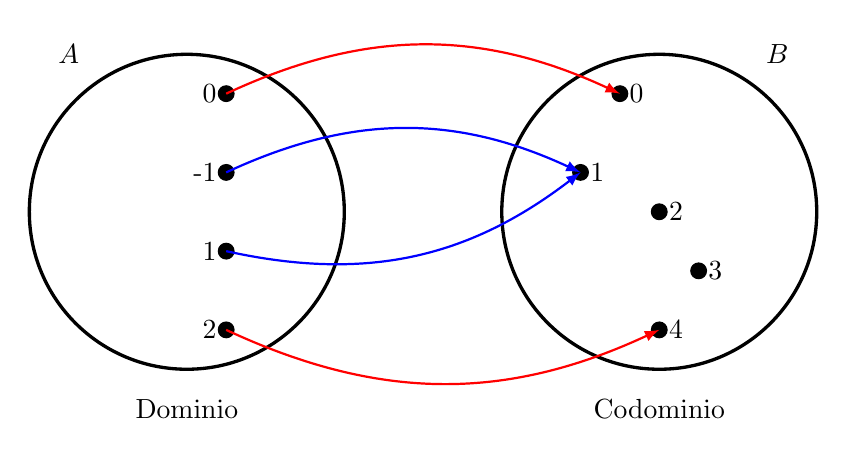
\begin{tikzpicture}[scale=1]
			% Coordenadas de puntos
			\coordinate (A0) at (0.5,1.5);
			\coordinate (Am1) at (.5,.5);
			\coordinate (A1) at (.5,-.5);
			\coordinate (A2) at (.5,-1.5);
			
			\coordinate (B0) at (5.5,1.5);
			\coordinate (B1) at (5,.5);
			\coordinate (B2) at (6,0);
			\coordinate (B3) at (6.5,-.75);
			\coordinate (B4) at (6,-1.5);
			
			% Circunferencias
			\node at (-1.5, 2) {$A$};
			\node at (7.5, 2) {$B$};
			\draw[very thick] (0,0) circle (2);
			\draw[very thick] (6,0) circle (2);
			\node at (0, -2.5) {Dominio};
			\node at (6, -2.5) {Codominio};
			
			% Puntos
			\draw[fill] (A0) circle (1mm) node[left] {0};
			\draw[fill] (Am1) circle (1mm) node[left] {-1};
			\draw[fill] (A1) circle (1mm) node[left] {1};
			\draw[fill] (A2) circle (1mm) node[left] {2};
			
			\draw[fill] (B0) circle (1mm) node[right] {0};
			\draw[fill] (B1) circle (1mm) node[right] {1};
			\draw[fill] (B2) circle (1mm) node[right] {2};
			\draw[fill] (B3) circle (1mm) node[right] {3};
			\draw[fill] (B4) circle (1mm) node[right] {4};
			
			% flechas
			\draw[red, thick, -latex] (A0) to [bend left = 25] (B0);
			\draw[blue, thick, -latex] (Am1) to [bend left = 25] (B1);
			\draw[blue, thick, -latex] (A1) to [bend left = -25] (B1);
			\draw[red, thick, -latex] (A2) to [bend left = -25] (B4);
		\end{tikzpicture}
	\end{figure}
\end{fmd-example}


\begin{fmd-definition}[Función] \index{función}
	$f$ es una función o aplicación de $A$ en $B$ si y sólo si $f$ es una relación
	entre $A$ y $B$ (en consecuencia, $f \subset A \times B$), tal que todo elemento de $A$ tiene un único correspondiente en $B$.
\end{fmd-definition}

\textbf{Observaciones}:
\begin{itemize}
	\item Si $(a, b) \in f$ decimos que $b$ es el correspondiente o \textit{imagen} de $a$,
	por $f$, y suele escribirse $b = f(a)$, en otras palabras, $b$ es el transformado de $a$
	por la función $f$.
	\item Si $f$ es como arriba, una aplicación o un \textit{mapeo} de $A$ a $B$ a menudo se escribe $x \mapsto f(x)$ para denotar la imagen de $x$ por $f$. Por ejemplo: Si $A = \R$ y  $B = \R^{+}$, sea $f: \R \rightarrow \R^{+}$ la aplicación $f(x) = x^2$, significa el mapeo cuyo valor en $x$ es $x^2$. Podemos también decir: $f$ es la aplicación tal que $x \mapsto x^2$ ($x$ se mapea a $x^2$ o $x$ se transforma en $x^2$ o $x$ se aplica a $x^2$). En este caso la imagen de $f$ es el conjunto de números reales no negativos.
	\item Una función queda especificada si se da el dominio $A$, el codominio $B$,
	y además la relación $f \subset A \times B$, que satisface las condiciones de la definición.
	\item Por ser un conjunto, $f$ puede estar dado por \textit{extensión}, como conjunto de pares ordenados, o bien por \textit{comprensión}, mediante una fórmula o ley de correspondencia que permita asignar a cada objeto del dominio su imagen en el codominio.
\end{itemize}%

\begin{fmd-example}[Funciones]
	Determinamos si las siguientes relaciones son funciones.
	\begin{enumerate}
		\item Sean $A =\{a,b,c,d\}, B=\{1,2,3\}$ y la relación:
		\[ f = \{(a, 1), (b, 2), (c,3), (d,1)\} \]
		Se cumplen las condiciones de la definición, y resulta $f$ una función tal que:
		\[ f(a) = 1, \quad f(b) = 2, \quad f(c)=2, \quad f(d)=1 \]
		
		\item Con los mismos $A$ y $B$ la relación
		\[ \{(a,1),(a,2),(b,2),(c,1)\} \]
		\textit{No es una función}.
		\begin{itemize}
			\item No todo elemento en $A$ ($d$) tiene imagen en $B$;
			\item Un mismo elemento en $A$ ($a$) tiene dos imágenes en $B$ (1 y 2).
		\end{itemize}
		El diagrama de la relación es:
		\begin{figure}[H]
			\centering
			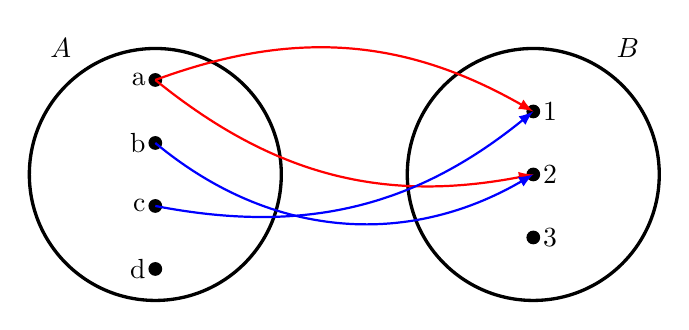
\begin{tikzpicture}[scale=.8]
				% Coordenadas de puntos
				\coordinate (a) at (0,1.5);
				\coordinate (b) at (0,.5);
				\coordinate (c) at (0,-.5);
				\coordinate (d) at (0,-1.5);
				
				\coordinate (B1) at (6,1);
				\coordinate (B2) at (6,0);
				\coordinate (B3) at (6,-1);
				
				% Circunferencias
				\node at (-1.5, 2) {$A$};
				\node at (7.5, 2) {$B$};
				\draw[very thick] (0,0) circle (2);
				\draw[very thick] (6,0) circle (2);
				
				% Puntos
				\draw[fill] (a) circle (1mm) node[left] {a};
				\draw[fill] (b) circle (1mm) node[left] {b};
				\draw[fill] (c) circle (1mm) node[left] {c};
				\draw[fill] (d) circle (1mm) node[left] {d};
				
				\draw[fill] (B1) circle (1mm) node[right] {1};
				\draw[fill] (B2) circle (1mm) node[right] {2};
				\draw[fill] (B3) circle (1mm) node[right] {3};
				
				% flechas
				\draw[red, thick, -latex] (a) to [bend left = 25] (B1);
				\draw[red, thick, -latex] (a) to [bend left = -25] (B2);
				\draw[blue, thick, -latex] (b) to [bend left = -35] (B2);
				\draw[blue, thick, -latex] (c) to [bend left = -25] (B1);
			\end{tikzpicture}
		\end{figure}
		
		\item Si $A$ es el conjunto de las personas y $f$ es la relación en $A$ definida por:
		\[(x, y) \in f \iff x \mbox{ es hijo de } y\]
		entonces $f$ es una función de $A$ en $A$, ya que toda persona tiene padre y
		este es único.
		
		En cambio la relación definida en el mismo $A$ mediante:
		\[ (x,y) \in f \iff x \mbox{ es padre de } y \]
		no es una función de $A$ en $A$, ya que existen en $A$ personas que no son padres,
		es decir, elementos del dominio que carecen de imagen en el codominio, por otra
		parte, tampoco se verifica la unicidad pues existen personas que son padres de más
		de un hijo.
	\end{enumerate}
\end{fmd-example}

\begin{lgnote}
	Si una relación es una función, la relación inversa no lo es necesariamente.
\end{lgnote}

\subsection{Representación cartesiana de funciones} \label{sec:cartesiano}

Las funciones pueden representarse mediante un sistema de coordenadas cartesianas
en el plano o en el espacio, según el dominio sea unidimensional o bidimensional
respectivamente. En el caso del plano, el dominio es un subconjunto del eje horizontal,
y el codominio, del eje vertical.

\begin{fmd-example} \label{frame:ejm2}
	Representación cartesiana de la función del ejemplo \ref{ex:funcion}.
	\[A = \{ -1, 0, 1, 2 \} \quad B = \{ 0, 1, 2, 3, 4 \}\]
	\[ f(x) = y = x^2 \]
	
	Si $g: \mathbb{R} \rightarrow \mathbb{R}^{+}_0 / g(x) = y = x^2$, resulta la parábola de la figura.
	
	\begin{figure}[H]
		\centering
		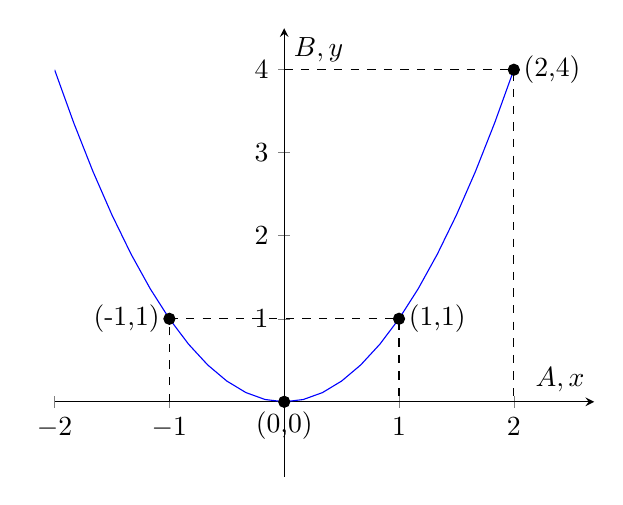
\begin{tikzpicture}[scale=1]
			\begin{axis}[domain=-2:2,
				y domain=0:4,
				ymin=-.9,
				xmax = 2.7,
				ymax = 4.5,
				axis lines = middle,
				xlabel = {$A, x$},
				ylabel = {$B, y$}]
				\addplot[blue] {x^2};
				\addplot [only marks] coordinates {(-1,1) (0,0) (1,1) (2,4)};
				\node [left] at (axis cs:-1,1) {(-1,1)};
				\node [below] at (axis cs:0,0) {(0,0)};
				\node [right] at (axis cs:1,1) {(1,1)};
				\node [right] at (axis cs:2,4) {(2,4)};
				\addplot[dashed] coordinates {(-1,0) (-1,1) (1,1) (1,0)};
				\addplot[dashed] coordinates {(0,4) (2,4) (2,0)};
			\end{axis}
		\end{tikzpicture}
		\label{fig:parabola}
	\end{figure}
\end{fmd-example}

\begin{fmd-example}
	Sea $f: \mathbb{Z} \rightarrow \mathbb{Z}$ tal que la imagen de cada entero es su
	opuesto aumentado en 1, es decir: $f(x) = -x + 1$.
	
	\begin{figure}[H]
		\centering
		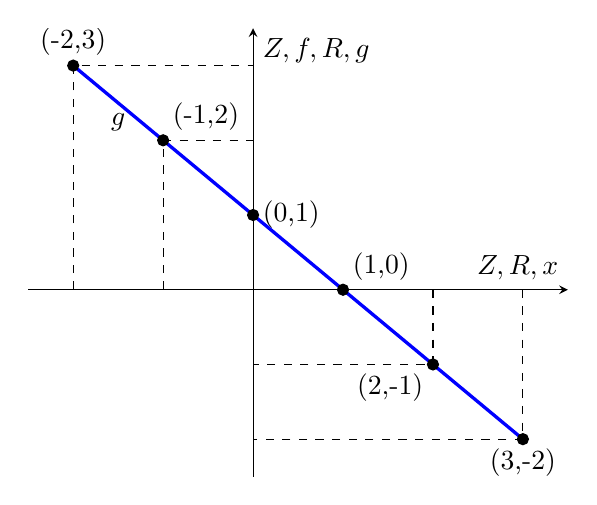
\begin{tikzpicture}[scale=1]
			\begin{axis}[domain=-2:3,
				y domain=-2:3,
				xmin=-2.5,
				ymin=-2.5,
				xmax = 3.5,
				ymax = 3.5,
				axis lines = middle,
				xlabel = {$Z, R, x$},
				ylabel = {$Z, f, R, g$},
				xtick=false, ytick=false]
				\addplot [only marks] coordinates {(-2,3) (-1,2) (0,1) (1,0) (2,-1)
					(3, -2)};
				\node [above] at (axis cs:-2,3) {(-2,3)};
				\node [above right] at (axis cs:-1,2) {(-1,2)};
				\node [right] at (axis cs:0,1) {(0,1)};
				\node [above right] at (axis cs:1,0) {(1,0)};
				\node [below left] at (axis cs:2,-1) {(2,-1)};
				\node [below] at (axis cs:3,-2) {(3,-2)};
				\addplot[dashed] coordinates {(-2,0) (-2,3) (0,3)};
				\addplot[dashed] coordinates {(-1,0) (-1,2) (0,2)};
				\addplot[dashed] coordinates {(2,0) (2,-1) (0,-1)};
				\addplot[dashed] coordinates {(3,0) (3,-2) (0,-2)};
				
				\addplot[very thick, blue] {-x+1} node[pos=.1, below, black] {$g$};
			\end{axis}
		\end{tikzpicture}
		\label{fig:recta}
	\end{figure}
	
	Si $g: \mathbb{R} \rightarrow \mathbb{R}$ es tal que $g(x) = -x + 1$. Su representación 
	es un conjunto continuo de $\mathbb{R}^2$, consistente en una recta del plano.
	
	Notar que $f \ne g$ aunque $f \subset g$.
\end{fmd-example}

\begin{example}[Función de dos variables]
	\
	
	Consideremos $A = \{1, 2\}$, $B = \{1,2,3,4\}$ y la función:
	\[ f: A^2 \rightarrow B \]
	que asigna a cada elemento del dominio $A^2$, la suma de sus componentes:
	\[ f(x, y) = x + y \]
	\begin{enumerate}
		\item Representación en una tabla de simple entrada.
		\begin{table}[H]
			\centering
			\begin{tabular}{c|c}
				$(x, y)$ & $f(x, y) = x + y$\\ \hline
				$(1,1)$ & 2\\
				$(1,2)$ & 3\\
				$(2,1)$ & 3\\
				$(2,2)$ & 4
			\end{tabular}
		\end{table}
		El elemento 1 de $B$ carece de antecedente o \gls{preimagen}\footnote{Ver definición \ref{def:preimagen}, pág. \pageref{def:preimagen}.}  en $A$.
	\end{enumerate}
	
	\begin{enumerate}
		\setcounter{enumi}{1}
		\item Representación en una tabla de doble entrada.
		\begin{table}[H]
			\centering
			\begin{tabular}{c|cc}
				$f$ & 1 & 2\\ \hline
				1 & 2 & 3\\
				2 & 3 & 4
			\end{tabular}
		\end{table}
		\item El diagrama de Venn es:
		\begin{figure}[H]
			\centering
			\begin{tikzpicture}[scale=1]
				% Coordenadas de puntos
				\coordinate (a) at (0,1.5);
				\coordinate (b) at (0,.5);
				\coordinate (c) at (0,-.5);
				\coordinate (d) at (0,-1.5);
				
				\coordinate (B1) at (6,1.5);
				\coordinate (B2) at (6,.5);
				\coordinate (B3) at (6,-.5);
				\coordinate (B4) at (6,-1.5);
				
				% Circunferencias
				\node at (-1.5, 2) {$A^2$};
				\node at (7.5, 2) {$B$};
				\draw[very thick] (0,0) circle (2);
				\draw[very thick] (6,0) circle (2);
				\draw[fill=black!20] (B3) ellipse (.6 and 1.5);
				\node at (0, -2.5) {Dominio};
				\node at (6, -2.5) {Codominio};
				\node at (8.8, -1.2) {Rango};
				\draw[latex-] ($(B3) + (.6,0)$) to [bend left = 20] (8,-1.1);
				
				% Puntos
				\draw[fill] (a) circle (1mm) node[left] {$(1,1)$};
				\draw[fill] (b) circle (1mm) node[left] {$(1,2)$};
				\draw[fill] (c) circle (1mm) node[left] {$(2,1)$};
				\draw[fill] (d) circle (1mm) node[left] {$(2,2)$};
				
				\draw[fill] (B1) circle (1mm) node[right] {1};
				\draw[fill] (B2) circle (1mm) node[right] {2};
				\draw[fill] (B3) circle (1mm) node[right] {3};
				\draw[fill] (B4) circle (1mm) node[right] {4};
				
				% flechas
				\draw[red, thick, -latex] (a) to [bend left = 25] (B2);
				\draw[red, thick, -latex] (b) to [bend left = 15] (B3);
				\draw[blue, thick, -latex] (c) to [bend left = -35] (B3);
				\draw[blue, thick, -latex] (d) to [bend left = -25] (B4);
			\end{tikzpicture}
		\end{figure}
	\end{enumerate}
	
	\begin{enumerate}
		\setcounter{enumi}{3}
		\item Representación cartesiana en el espacio.
		\begin{figure}[H]
			\centering
			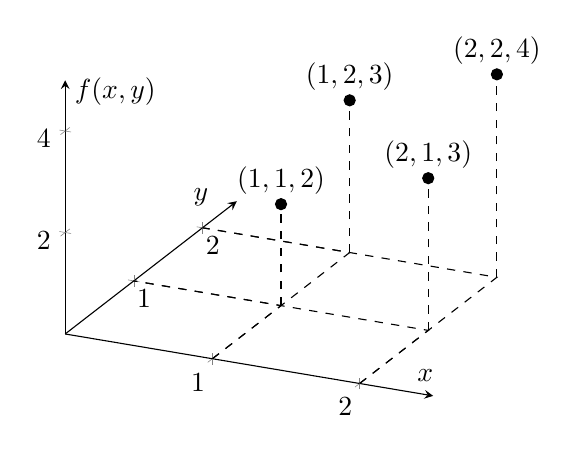
\begin{tikzpicture}[scale=1]
				\begin{axis}[axis lines = middle,
					xmin=0, xmax=2.5,
					ymin=0, ymax=2.5, zmax=5,
					xlabel={$x$}, ylabel={$y$}, zlabel={$f(x,y)$}]
					\addplot3[only marks] coordinates {(1,1,2) (1,2,3) (2,1,3) (2,2,4)};
					\addplot3[dashed] coordinates {(1,0,0) (1,1,0) (0,1,0)};
					\addplot3[dashed] coordinates {(1,1,0) (1,1,2)} node[above] {$(1,1,2)$};
					\addplot3[dashed] coordinates {(1,0,0) (1,2,0) (0,2,0)};
					\addplot3[dashed] coordinates {(1,2,0) (1,2,3)} node[above] {$(1,2,3)$};
					\addplot3[dashed] coordinates {(2,0,0) (2,1,0) (0,1,0)};
					\addplot3[dashed] coordinates {(2,1,0) (2,1,3)} node[above] {$(2,1,3)$};
					\addplot3[dashed] coordinates {(2,0,0) (2,2,0) (0,2,0)};
					\addplot3[dashed] coordinates {(2,2,0) (2,2,4)} node[above] {$(2,2,4)$};
				\end{axis}
			\end{tikzpicture}
		\end{figure}
	\end{enumerate}
	
	\begin{enumerate}
		\setcounter{enumi}{4}
		\item La misma función puede representarse de la siguiente manera, desconectando
		el dominio del codominio.
		\begin{figure}[H]
			\centering
			\begin{tikzpicture}[scale=1]
				% Puntos
				\coordinate (a) at (1,1);
				\coordinate (b) at (2,1);
				\coordinate (c) at (1,2);
				\coordinate (d) at (2,2);
				
				\coordinate (r) at (4,.2);
				\coordinate (B1) at ($(r) + (1,1)$);
				\coordinate (B2) at ($(r) + (2,2)$);
				\coordinate (B3) at ($(r) + (3,3)$);
				\coordinate (B4) at ($(r) + (4,4)$);
				
				% Ejes
				\draw[-latex] (-1,0) -- (3,0) node[below]{$x$};
				\node[below] at (1,0) {1};
				\node[below] at (2,0) {2};
				\node[left] at (0,1) {1};
				\node[left] at (0,2) {2};
				\draw[-latex] (0,-1) -- (0,3) node[left]{$y$};
				
				% Puntos
				\draw[fill] (a) circle (2pt);
				\draw[fill] (b) circle (2pt);
				\draw[fill] (c) circle (2pt);
				\draw[fill] (d) circle (2pt);
				
				% Dashes
				\draw[dashed] (1, 0) -- (1, 3); 
				\draw[dashed] (2, 0) -- (2, 3); 
				\draw[dashed] (0, 1) -- (3, 1); 
				\draw[dashed] (0, 2) -- (3, 2);
				
				% Circunferencia
				\draw[blue] (1.5,1.5) circle (1);
				\node[right] at (.3,2.5) {$A^2$};
				
				% Recta
				\draw[red, very thick, -latex] (4, .2) -- (8.5, 4.7) node[left, pos=.98]
				{$B$};
				\draw[fill] (B1) circle (2pt) node[right]{1};
				\draw[fill] (B2) circle (2pt) node[right]{2};
				\draw[fill] (B3) circle (2pt) node[right]{3};
				\draw[fill] (B4) circle (2pt) node[right]{4};
				
				% flechas
				\draw[-latex] (a) to [bend left = 25] (B2);
				\draw[-latex] (b) to [bend left = 15] (B3);
				\draw[-latex] (c) to [bend left = 25] (B3);
				\draw[-latex] (d) to [bend left = 25] (B4);
			\end{tikzpicture}
		\end{figure}
	\end{enumerate}
\end{example}

\subsection{Clasificación de funciones} \label{sec:clasif}
Sea una función $f: A \rightarrow B$
\begin{itemize}
	\item Si ocurre que elementos distintos del dominio tienen imágenes distintas 
	en el codominio, entonces $f$ se llama \gls{funcioninyectiva} o uno a uno.
	\index{función!inyectiva}
	\item Por otra parte, si todo elemento del codominio es imagen de algún elemento 
	del dominio, se llama \gls{funcionsobreyectiva}. \index{función!sobreyectiva}
	\item Cuando se presentan ambas situaciones simultáneamente, se llama \gls{funcionbiyectiva} o correspondencia biunívoca. \index{función!biyectiva}
\end{itemize}

\subsubsection{Función inyectiva}
\vspace{1em} \index{función!inyectiva}
\begin{fmd-definition}[Función inyectiva]
	Una función $f: A \rightarrow B$ es inyectiva si, y solo si, para cualquier par de elementos distintos $x'$ y $x''$ en el conjunto $A$, sus imágenes bajo la función $f$ también son distintas.
\end{fmd-definition}
\vspace{1mm}

O, de forma equivalente:

Una función $f: A \rightarrow B$ es inyectiva si, y solo si, cuando dos elementos cualesquiera $x', x'' \in A$ tienen la misma imagen, $f(x') = f(x'')$ entonces esos dos elementos deben ser el mismo elemento ($x' = x''$).

\begin{itemize}
	\item En la inyectividad no puede darse que elementos distintos del dominio den la misma
	imagen, fig. \ref{fig:inyectiva_discreta}.
	\item En el diagrama de Venn no puede presentarse ninguna bifurcación de elementos del 
	dominio hacia el codominio.
	\item En la representación plana cartesiana no puede ocurrir que una ordenada
	corresponda a más de una abscisa, fig. \ref{fig:inyectiva_continua}.
\end{itemize}

% TODO: pasar cada gráfica a standalone para llamarlas y referenciarlas independientemente.
\begin{figure}[H]
	\centering
	\begin{minipage}{.3\textwidth}
		\centering
		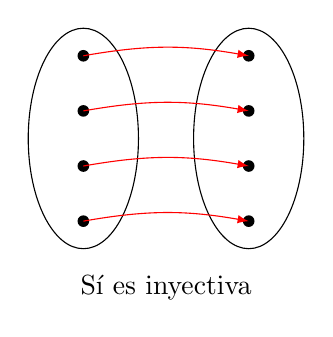
\begin{tikzpicture}[scale=.7]
			% Coordenadas
			\coordinate (A) at (0,0);
			\coordinate (A1) at (0,1.5);
			\coordinate (A2) at (0,.5);
			\coordinate (A3) at (0,-.5);
			\coordinate (A4) at (0,-1.5);
			
			\coordinate (B) at (3,0);
			\coordinate (B1) at (3,1.5);
			\coordinate (B2) at (3,.5);
			\coordinate (B3) at (3,-.5);
			\coordinate (B4) at (3,-1.5);
			
			% Elipses
			\draw[] (A) ellipse (1 and 2);
			\draw[] (B) ellipse (1 and 2);
			
			% Elementos
			\fill[black] (A1) circle (3pt);
			\fill[black] (A2) circle (3pt);
			\fill[black] (A3) circle (3pt);
			\fill[black] (A4) circle (3pt);
			
			\fill[black] (B1) circle (3pt);
			\fill[black] (B2) circle (3pt);
			\fill[black] (B3) circle (3pt);
			\fill[black] (B4) circle (3pt);
			
			% Flechas
			\draw[-latex, red] (A1) to [bend left = 10] (B1);
			\draw[-latex, red] (A2) to [bend left = 10] (B2);
			\draw[-latex, red] (A3) to [bend left = 10] (B3);
			\draw[-latex, red] (A4) to [bend left = 10] (B4);
			
			% Caption
			\node at (1.5,-2.7) {Sí es inyectiva};
		\end{tikzpicture}
	\end{minipage}
	\begin{minipage}{.3\textwidth}
		\centering
		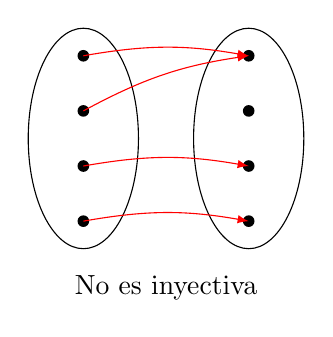
\begin{tikzpicture}[scale=.7]
			% Coordenadas
			\coordinate (A) at (0,0);
			\coordinate (A1) at (0,1.5);
			\coordinate (A2) at (0,.5);
			\coordinate (A3) at (0,-.5);
			\coordinate (A4) at (0,-1.5);
			
			\coordinate (B) at (3,0);
			\coordinate (B1) at (3,1.5);
			\coordinate (B2) at (3,.5);
			\coordinate (B3) at (3,-.5);
			\coordinate (B4) at (3,-1.5);
			
			% Elipses
			\draw[] (A) ellipse (1 and 2);
			\draw[] (B) ellipse (1 and 2);
			
			% Elementos
			\fill[black] (A1) circle (3pt);
			\fill[black] (A2) circle (3pt);
			\fill[black] (A3) circle (3pt);
			\fill[black] (A4) circle (3pt);
			
			\fill[black] (B1) circle (3pt);
			\fill[black] (B2) circle (3pt);
			\fill[black] (B3) circle (3pt);
			\fill[black] (B4) circle (3pt);
			
			% Flechas
			\draw[-latex, red] (A1) to [bend left = 10] (B1);
			\draw[-latex, red] (A2) to [bend left = 10] (B1);
			\draw[-latex, red] (A3) to [bend left = 10] (B3);
			\draw[-latex, red] (A4) to [bend left = 10] (B4);
			
			% Caption
			\node at (1.5,-2.7) {No es inyectiva};
		\end{tikzpicture}
	\end{minipage}
	\begin{minipage}{.3\textwidth}
		\centering
		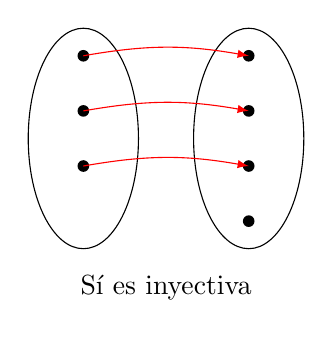
\begin{tikzpicture}[scale=.7]
			% Coordenadas
			\coordinate (A) at (0,0);
			\coordinate (A1) at (0,1.5);
			\coordinate (A2) at (0,.5);
			\coordinate (A3) at (0,-.5);
			
			\coordinate (B) at (3,0);
			\coordinate (B1) at (3,1.5);
			\coordinate (B2) at (3,.5);
			\coordinate (B3) at (3,-.5);
			\coordinate (B4) at (3,-1.5);
			
			% Elipses
			\draw[] (A) ellipse (1 and 2);
			\draw[] (B) ellipse (1 and 2);
			
			% Elementos
			\fill[black] (A1) circle (3pt);
			\fill[black] (A2) circle (3pt);
			\fill[black] (A3) circle (3pt);
			
			\fill[black] (B1) circle (3pt);
			\fill[black] (B2) circle (3pt);
			\fill[black] (B3) circle (3pt);
			\fill[black] (B4) circle (3pt);
			
			% Flechas
			\draw[-latex, red] (A1) to [bend left = 10] (B1);
			\draw[-latex, red] (A2) to [bend left = 10] (B2);
			\draw[-latex, red] (A3) to [bend left = 10] (B3);
			
			% Caption
			\node at (1.5,-2.7) {Sí es inyectiva};
		\end{tikzpicture}
	\end{minipage}
	\caption{Identificación de funciones inyectivas discretas}
	\label{fig:inyectiva_discreta}
\end{figure}

\begin{figure}[H]
	\centering
	\begin{minipage}{.45\textwidth}
		\centering
		\begin{figure}[H]
			\centering
			\begin{tikzpicture}[scale=.5]
				\begin{axis}[axis lines=middle, xticklabels={}, yticklabels={}]
					\addplot[blue, very thick] {x^3};
				\end{axis}
			\end{tikzpicture}
			\caption*{$f:\mathbb{R} \rightarrow \mathbb{R} / f(x) = x^3$\\Sí es inyectiva}
		\end{figure}
	\end{minipage}
	\begin{minipage}{.45\textwidth}
		\centering
		\begin{figure}[H]
			\centering
			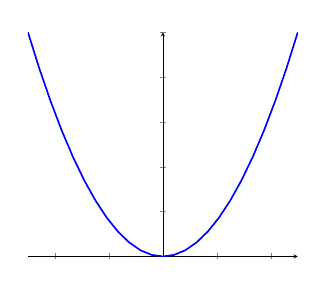
\begin{tikzpicture}[scale=.5]
				\begin{axis}[axis lines=middle, xticklabels={}, yticklabels={}]
					\addplot[blue, very thick] {x^2};
				\end{axis}
			\end{tikzpicture}
			\caption*{$f:\mathbb{R} \rightarrow \mathbb{R}_0^{+} / f(x) = x^2$\\No es inyectiva}
		\end{figure}
	\end{minipage}
	\caption{Identificación de funciones inyectivas continuas.}
	\label{fig:inyectiva_continua}
\end{figure}

\subsubsection{Función sobreyectiva} \index{función!sobreyectiva}
\vspace{1em}
\begin{fmd-definition}[Función sobreyectiva]
	Una función $f: A \rightarrow B$ es \textit{sobreyectiva} si, y solo si, para cada elemento $y \in B$, existe al menos un elemento $x \in A$ tal que $y = f(x)$.
\end{fmd-definition}
\begin{itemize}
	\item El conjunto de las imágenes (\gls{rango} o \textit{recorrido}) \index{rango} se identifica con el codominio de la función. No hay elementos del codominio que no sea la imagen de \textit{al menos un} elemento del dominio, en otras palabras, el rango y el codominio coinciden, figs. \ref{fig:sobreyectiva_discreta} y \ref{fig:sobreyectiva_continua}.
	\item Es usual nombrar a las funciones sobreyectivas como ``sobre'' o ``suryectiva''
\end{itemize}

\begin{figure}[H]
	\begin{minipage}{.32\textwidth}
		\centering
		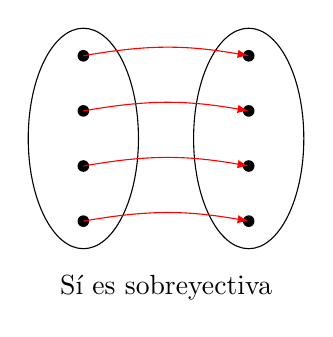
\begin{tikzpicture}[scale=.7]
			% Coordenadas
			\coordinate (A) at (0,0);
			\coordinate (A1) at (0,1.5);
			\coordinate (A2) at (0,.5);
			\coordinate (A3) at (0,-.5);
			\coordinate (A4) at (0,-1.5);
			
			\coordinate (B) at (3,0);
			\coordinate (B1) at (3,1.5);
			\coordinate (B2) at (3,.5);
			\coordinate (B3) at (3,-.5);
			\coordinate (B4) at (3,-1.5);
			
			% Elipses
			\draw[] (A) ellipse (1 and 2);
			\draw[] (B) ellipse (1 and 2);
			
			% Elementos
			\fill[black] (A1) circle (3pt);
			\fill[black] (A2) circle (3pt);
			\fill[black] (A3) circle (3pt);
			\fill[black] (A4) circle (3pt);
			
			\fill[black] (B1) circle (3pt);
			\fill[black] (B2) circle (3pt);
			\fill[black] (B3) circle (3pt);
			\fill[black] (B4) circle (3pt);
			
			% Flechas
			\draw[-latex, red] (A1) to [bend left = 10] (B1);
			\draw[-latex, red] (A2) to [bend left = 10] (B2);
			\draw[-latex, red] (A3) to [bend left = 10] (B3);
			\draw[-latex, red] (A4) to [bend left = 10] (B4);
			
			% Caption
			\node at (1.5,-2.7) {Sí es sobreyectiva};
		\end{tikzpicture}
	\end{minipage}
	\begin{minipage}{.32\textwidth}
		\centering
		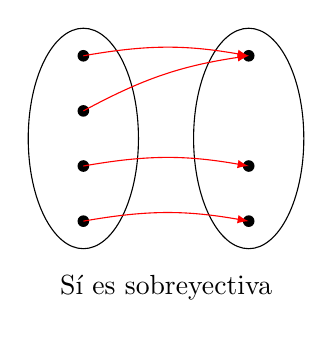
\begin{tikzpicture}[scale=.7]
			% Coordenadas
			\coordinate (A) at (0,0);
			\coordinate (A1) at (0,1.5);
			\coordinate (A2) at (0,.5);
			\coordinate (A3) at (0,-.5);
			\coordinate (A4) at (0,-1.5);
			
			\coordinate (B) at (3,0);
			\coordinate (B1) at (3,1.5);
			\coordinate (B2) at (3,.5);
			\coordinate (B3) at (3,-.5);
			\coordinate (B4) at (3,-1.5);
			
			% Elipses
			\draw[] (A) ellipse (1 and 2);
			\draw[] (B) ellipse (1 and 2);
			
			% Elementos
			\fill[black] (A1) circle (3pt);
			\fill[black] (A2) circle (3pt);
			\fill[black] (A3) circle (3pt);
			\fill[black] (A4) circle (3pt);
			
			\fill[black] (B1) circle (3pt);
			%\fill[black] (B2) circle (3pt);
			\fill[black] (B3) circle (3pt);
			\fill[black] (B4) circle (3pt);
			
			% Flechas
			\draw[-latex, red] (A1) to [bend left = 10] (B1);
			\draw[-latex, red] (A2) to [bend left = 10] (B1);
			\draw[-latex, red] (A3) to [bend left = 10] (B3);
			\draw[-latex, red] (A4) to [bend left = 10] (B4);
			
			% Caption
			\node at (1.5,-2.7) {Sí es sobreyectiva};
		\end{tikzpicture}
	\end{minipage}
	\begin{minipage}{.32\textwidth}
		\centering
		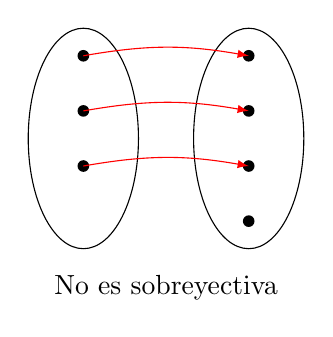
\begin{tikzpicture}[scale=.7]
			% Coordenadas
			\coordinate (A) at (0,0);
			\coordinate (A1) at (0,1.5);
			\coordinate (A2) at (0,.5);
			\coordinate (A3) at (0,-.5);
			
			\coordinate (B) at (3,0);
			\coordinate (B1) at (3,1.5);
			\coordinate (B2) at (3,.5);
			\coordinate (B3) at (3,-.5);
			\coordinate (B4) at (3,-1.5);
			
			% Elipses
			\draw[] (A) ellipse (1 and 2);
			\draw[] (B) ellipse (1 and 2);
			
			% Elementos
			\fill[black] (A1) circle (3pt);
			\fill[black] (A2) circle (3pt);
			\fill[black] (A3) circle (3pt);
			
			\fill[black] (B1) circle (3pt);
			\fill[black] (B2) circle (3pt);
			\fill[black] (B3) circle (3pt);
			\fill[black] (B4) circle (3pt);
			
			% Flechas
			\draw[-latex, red] (A1) to [bend left = 10] (B1);
			\draw[-latex, red] (A2) to [bend left = 10] (B2);
			\draw[-latex, red] (A3) to [bend left = 10] (B3);
			
			% Caption
			\node at (1.5,-2.7) {No es sobreyectiva};
		\end{tikzpicture}
	\end{minipage}
	\caption{Función sobreyectiva, caso discreto.}
	\label{fig:sobreyectiva_discreta}
\end{figure}

\begin{figure}[H]
	\centering
	\begin{minipage}{.45\textwidth}
		\centering
		\begin{figure}[H]
			\centering
			\begin{tikzpicture}[scale=.5]
				\begin{axis}[axis lines=middle, xticklabels={}, yticklabels={}]
					\addplot[blue, very thick] {x^3};
				\end{axis}
			\end{tikzpicture}
			\caption*{$f:\mathbb{R} \rightarrow \mathbb{R} / f(x) = x^3$\\Sí es sobreyectiva}
		\end{figure}
	\end{minipage}
	\begin{minipage}{.45\textwidth}
		\centering
		\begin{figure}[H]
			\centering
			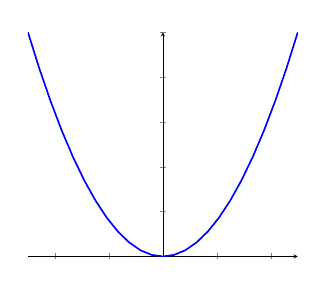
\begin{tikzpicture}[scale=.5]
				\begin{axis}[axis lines=middle, xticklabels={}, yticklabels={}]
					\addplot[blue, very thick] {x^2};
				\end{axis}
			\end{tikzpicture}
			\caption*{$f:\mathbb{R} \rightarrow \mathbb{R}_0^{+} / f(x) = x^2$\\Sí es sobreyectiva}
		\end{figure}
	\end{minipage}
	\caption{Ejemplos de funciones sobreyectivas continuas.}
	\label{fig:sobreyectiva_continua}
\end{figure}

\subsubsection{Función biyectiva}
\vspace{1em} \index{función!biyectiva}
\begin{fmd-definition}[Función biyectiva]
	$f:A \rightarrow B \mbox{ es biyectiva si } f \mbox{ es inyectiva y sobreyectiva}$.
\end{fmd-definition}

\begin{lgnote}
	Si $f: A \rightarrow B$ no es biyectiva, entonces no es inyectiva o no es sobreyectiva, figuras \ref{fig:biyectiva_discreta} y \ref{fig:biyectiva_continua}.
\end{lgnote}

\begin{figure}[H]
	\centering
	\begin{minipage}{.32\textwidth}
		\centering
		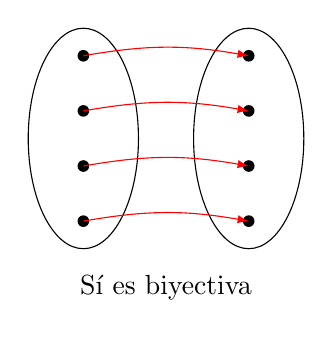
\begin{tikzpicture}[scale=.7]
			% Coordenadas
			\coordinate (A) at (0,0);
			\coordinate (A1) at (0,1.5);
			\coordinate (A2) at (0,.5);
			\coordinate (A3) at (0,-.5);
			\coordinate (A4) at (0,-1.5);
			
			\coordinate (B) at (3,0);
			\coordinate (B1) at (3,1.5);
			\coordinate (B2) at (3,.5);
			\coordinate (B3) at (3,-.5);
			\coordinate (B4) at (3,-1.5);
			
			% Elipses
			\draw[] (A) ellipse (1 and 2);
			\draw[] (B) ellipse (1 and 2);
			
			% Elementos
			\fill[black] (A1) circle (3pt);
			\fill[black] (A2) circle (3pt);
			\fill[black] (A3) circle (3pt);
			\fill[black] (A4) circle (3pt);
			
			\fill[black] (B1) circle (3pt);
			\fill[black] (B2) circle (3pt);
			\fill[black] (B3) circle (3pt);
			\fill[black] (B4) circle (3pt);
			
			% Flechas
			\draw[-latex, red] (A1) to [bend left = 10] (B1);
			\draw[-latex, red] (A2) to [bend left = 10] (B2);
			\draw[-latex, red] (A3) to [bend left = 10] (B3);
			\draw[-latex, red] (A4) to [bend left = 10] (B4);
			
			% Caption
			\node at (1.5,-2.7) {Sí es biyectiva};
		\end{tikzpicture}
	\end{minipage}
	\begin{minipage}{.32\textwidth}
		\centering
		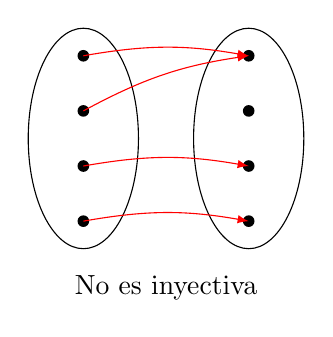
\begin{tikzpicture}[scale=.7]
			% Coordenadas
			\coordinate (A) at (0,0);
			\coordinate (A1) at (0,1.5);
			\coordinate (A2) at (0,.5);
			\coordinate (A3) at (0,-.5);
			\coordinate (A4) at (0,-1.5);
			
			\coordinate (B) at (3,0);
			\coordinate (B1) at (3,1.5);
			\coordinate (B2) at (3,.5);
			\coordinate (B3) at (3,-.5);
			\coordinate (B4) at (3,-1.5);
			
			% Elipses
			\draw[] (A) ellipse (1 and 2);
			\draw[] (B) ellipse (1 and 2);
			
			% Elementos
			\fill[black] (A1) circle (3pt);
			\fill[black] (A2) circle (3pt);
			\fill[black] (A3) circle (3pt);
			\fill[black] (A4) circle (3pt);
			
			\fill[black] (B1) circle (3pt);
			\fill[black] (B2) circle (3pt);
			\fill[black] (B3) circle (3pt);
			\fill[black] (B4) circle (3pt);
			
			% Flechas
			\draw[-latex, red] (A1) to [bend left = 10] (B1);
			\draw[-latex, red] (A2) to [bend left = 10] (B1);
			\draw[-latex, red] (A3) to [bend left = 10] (B3);
			\draw[-latex, red] (A4) to [bend left = 10] (B4);
			
			% Caption
			\node at (1.5,-2.7) {No es inyectiva};
		\end{tikzpicture}
	\end{minipage}
	\begin{minipage}{.32\textwidth}
		\centering
		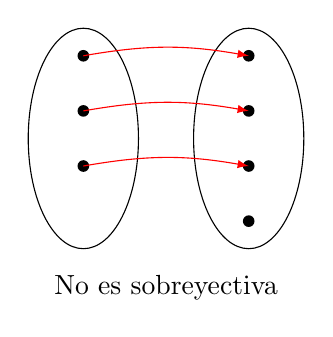
\begin{tikzpicture}[scale=.7]
			% Coordenadas
			\coordinate (A) at (0,0);
			\coordinate (A1) at (0,1.5);
			\coordinate (A2) at (0,.5);
			\coordinate (A3) at (0,-.5);
			
			\coordinate (B) at (3,0);
			\coordinate (B1) at (3,1.5);
			\coordinate (B2) at (3,.5);
			\coordinate (B3) at (3,-.5);
			\coordinate (B4) at (3,-1.5);
			
			% Elipses
			\draw[] (A) ellipse (1 and 2);
			\draw[] (B) ellipse (1 and 2);
			
			% Elementos
			\fill[black] (A1) circle (3pt);
			\fill[black] (A2) circle (3pt);
			\fill[black] (A3) circle (3pt);
			
			\fill[black] (B1) circle (3pt);
			\fill[black] (B2) circle (3pt);
			\fill[black] (B3) circle (3pt);
			\fill[black] (B4) circle (3pt);
			
			% Flechas
			\draw[-latex, red] (A1) to [bend left = 10] (B1);
			\draw[-latex, red] (A2) to [bend left = 10] (B2);
			\draw[-latex, red] (A3) to [bend left = 10] (B3);
			
			% Caption
			\node at (1.5,-2.7) {No es sobreyectiva};
		\end{tikzpicture}
	\end{minipage}
	\caption{Identificación de función biyectiva discreta.}
	\label{fig:biyectiva_discreta}
\end{figure}

\begin{figure}[H]
	\centering
	\begin{minipage}{.45\textwidth}
		\centering
		\begin{figure}[H]
			\centering
			\begin{tikzpicture}[scale=.5]
				\begin{axis}[axis lines=middle, xticklabels={}, yticklabels={}]
					\addplot[blue, very thick] {x^3};
				\end{axis}
			\end{tikzpicture}
			\caption*{$f:\mathbb{R} \rightarrow \mathbb{R} / f(x) = x^3$\\Sí es biyectiva}
		\end{figure}
	\end{minipage}
	\begin{minipage}{.45\textwidth}
		\centering
		\begin{figure}[H]
			\centering
			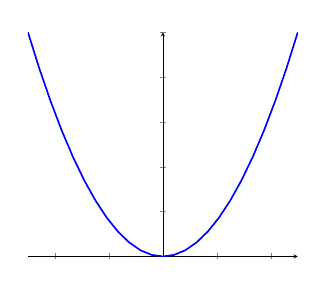
\begin{tikzpicture}[scale=.5]
				\begin{axis}[axis lines=middle, xticklabels={}, yticklabels={}]
					\addplot[blue, very thick] {x^2};
				\end{axis}
			\end{tikzpicture}
			\caption*{$f:\mathbb{R} \rightarrow \mathbb{R}_0^{+} / f(x) = x^2$\\No es biyectiva}
		\end{figure}
	\end{minipage}
	\caption{Función biyectiva continua.}
	\label{fig:biyectiva_continua}
\end{figure}

\begin{fmd-example}
	Probar la inyectividad de $f$, siendo $ f: \mathbb{N} \rightarrow \mathbb{N} \mbox{ tal que } f(x) = 2x$
	\begin{figure}[H]
		\centering
		\begin{tikzpicture}[scale=1]
			\begin{axis}[axis lines=middle, xmin=0, xmax=4.5,
				ymin=0, ymax=4.5, xlabel={$\mathbb{N}$}, ylabel={$\mathbb{N}$}]
				
				% Verticales
				\addplot[dashed] coordinates {(1,0) (1,4)};
				\addplot[dashed] coordinates {(2,0) (2,4)};
				\addplot[dashed] coordinates {(3,0) (3,4)};
				\addplot[dashed] coordinates {(4,0) (4,4)};
				
				% Horizontales
				\addplot[dashed] coordinates {(0,1) (4,1)};
				\addplot[dashed] coordinates {(0,2) (4,2)};
				\addplot[dashed] coordinates {(0,3) (4,3)};
				\addplot[dashed] coordinates {(0,4) (4,4)};
				
				% Puntos
				\addplot[only marks, mark size=4pt] coordinates {(1,2) (2,4)};
			\end{axis}
		\end{tikzpicture}
	\end{figure}
	\begin{itemize}
		\item Sean $x'$ y $x''$ en $\mathbb{N}$ tales que $f(x') = f(x'')$, entonces
		$2x' = 2 x''$, en consecuencia $x'= x''$. De modo que $f$ es inyectiva uno a uno.
		\item $f$ no es sobreyectiva, pues los elementos impares del codominio, carecen
		de antecedente. Resulta que $f$ no es biyectiva.
	\end{itemize}
	Si se utiliza el conjunto $P$ de los números naturales pares y
	$ f: \mathbb{N} \rightarrow \mathbb{P} \mbox{ tal que } f(x) = 2x$, $f$ resulta
	biyectiva.
\end{fmd-example}

\begin{fmd-example}
	Sean $A = \{ 1,2,3 \}$ y $B = \{ 1,2 \}$.
	
	Definimos $f: P(A) \rightarrow P(B)$ mediante $f(X) = X \cap B$, la imagen
	de todo subconjunto de $A$ es su intersección con $B$.
	
	El diagrama muestra que $f$ es sobreyectiva pero no inyectiva.
	
	\begin{figure}[H]
		\centering
		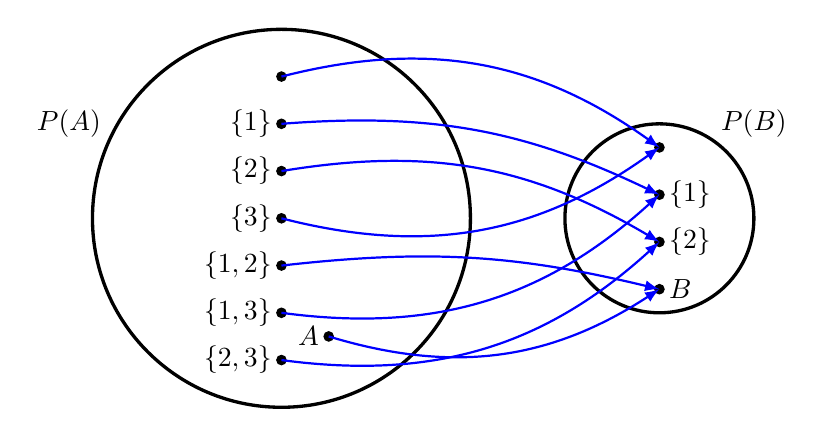
\begin{tikzpicture}[scale=.6]
			% Coordenadas de puntos
			\coordinate (a) at (0,3);
			\coordinate (b) at (0,2);
			\coordinate (c) at (0,1);
			\coordinate (d) at (0,0);
			\coordinate (e) at (0,-1);
			\coordinate (f) at (0,-2);
			\coordinate (g) at (0,-3);
			\coordinate (h) at (1,-2.5);
			
			\coordinate (B1) at (8,1.5);
			\coordinate (B2) at (8,.5);
			\coordinate (B3) at (8,-.5);
			\coordinate (B4) at (8,-1.5);
			
			% Circunferencias
			\node at (-4.5, 2) {$P(A)$};
			\node at (10, 2) {$P(B)$};
			\draw[very thick] (0,0) circle (4);
			\draw[very thick] (8,0) circle (2);
			
			% Puntos
			\draw[fill] (a) circle (1mm) node[left] {$\varnothing$};
			\draw[fill] (b) circle (1mm) node[left] {$\{1\}$};
			\draw[fill] (c) circle (1mm) node[left] {$\{2\}$};
			\draw[fill] (d) circle (1mm) node[left] {$\{3\}$};
			\draw[fill] (e) circle (1mm) node[left] {$\{1,2\}$};
			\draw[fill] (f) circle (1mm) node[left] {$\{1,3\}$};
			\draw[fill] (g) circle (1mm) node[left] {$\{2,3\}$};
			\draw[fill] (h) circle (1mm) node[left] {$A$};
			
			\draw[fill] (B1) circle (1mm) node[right] {$\varnothing$};
			\draw[fill] (B2) circle (1mm) node[right] {$\{1\}$};
			\draw[fill] (B3) circle (1mm) node[right] {$\{2\}$};
			\draw[fill] (B4) circle (1mm) node[right] {$B$};
			
			% flechas
			\draw[blue, thick, -latex] (a) to [bend left = 25] (B1);
			\draw[blue, thick, -latex] (b) to [bend left = 15] (B2);
			\draw[blue, thick, -latex] (c) to [bend left = 20] (B3);
			\draw[blue, thick, -latex] (d) to [bend left = -25] (B1);
			\draw[blue, thick, -latex] (e) to [bend left = 10] (B4);
			\draw[blue, thick, -latex] (f) to [bend left = -25] (B2);
			\draw[blue, thick, -latex] (g) to [bend left = -25] (B3);
			\draw[blue, thick, -latex] (h) to [bend left = -25] (B4);
		\end{tikzpicture}
	\end{figure}
\end{fmd-example}

\begin{fmd-example}[Función biyectiva]
	Sea $f: \mathbb{R} \rightarrow \mathbb{R}$ definida por $f(x) = x^3$.
	\begin{enumerate}
		\item $f$ es 1-1. En efecto, sean $x_1$ y $x_2$ en $\mathbb{R}$ tales que
		$f(x_1) = f(x_2)$, esto significa: $x_1^3 = x_2^3$, o $x_1^3 - x_2^3 = 0$,
		factorizando: \[(x_1 - x_2)(x_1^2 + x_1x_2 + x_2^2) = 0\]
		\[ x_1 - x_2 = 0 \implies x_1 = x_2 \]
		de $x_1^2 + x_1x_2 + x_2^2=0$ se tiene:
		\[ x_1 = \frac{-x_2 \pm \sqrt{x_2^2 - 4 x_2} }{2} =
		\frac{-x_2 \pm \sqrt{-3x_2^2}}{2} \]
		De donde:
		\begin{equation} \label{eq:x1}
			x_1 = \left( -\frac{1}{2} \pm i \frac{\sqrt{3}}{2} \right) x_2
		\end{equation}
		Si $x_2=0$ entonces $x_1 = 0$ y resulta $x_1 = x_2$, los cuales son los únicos
		valores reales que satisfacen \eqref{eq:x1}, en consecuencia $f$ \textbf{es inyectiva}.
		
		\item $f$ \textbf{es sobreyectiva}, pues
		\[ \forall y \in \mathbb{R}, \exists \ x = \sqrt[3]{y} \mbox{ tal que }
		f(x) = f(\sqrt[3]{y}) = \left( \sqrt[3]{y} \right)^3 = y\]
		Ocurre entonces que $f$ \textbf{es biyectiva}.
	\end{enumerate}
\end{fmd-example}

\subsection{Funciones especiales} \label{sec:especiales}
\index{funciones!especiales}
\begin{itemize}
	\item \textbf{Función constante} \index{función!constante}
	
	La función $f: A \rightarrow B$, que asigna a todos los elementos del dominio el
	elemento $b \in B$, se llama constante.
	
	Está definida por $f(x) = b$ para todo $x \in A$, se tiene:
	\[ f = \{ (x, b) / x \in A \} \]
	
	A menos que $A$ sea unitario, la función constante \textbf{no es inyectiva}, y
	\textbf{es sobreyectiva} si $B$ se reduce a un único elemento, fig. \ref{fig:funcion_constante}.
\end{itemize}
\begin{figure}[H]
	\centering
	\begin{tikzpicture}
		\begin{axis}[axis lines=middle, xlabel={$A$}, ylabel={$B$},
			xticklabels={}, yticklabels={}, ymin=-.5, ymax=2.5,
			scale=.6, xmin=-2.5, xmax=2.5]
			\addplot[thick] coordinates {(-2, 1) (2,1)};
			\node[above] at (40, 150) {$b$};
		\end{axis}
	\end{tikzpicture}
	\caption{Función constante}
	\label{fig:funcion_constante}
\end{figure}

\begin{itemize}
	\item \textbf{Función identidad} \index{función!identidad}
	
	Identidad en $A$ es la aplicación que asigna a cada elemento de $A$ el mismo elemento.
	$ i_A: A \rightarrow A \mbox{ tal que } i_A(x) = x$.
	
	A veces se utiliza el símbolo $\mathbf{1}_A$.
	
	Se tiene: $i_A = \{ (x, x) / x \in A \}$
	
	La identidad en $A$ es la diagonal de $A^2$. Como relación es reflexiva,
	simétrica y transitiva, o sea, de equivalencia en $A$; además es antisimétrica.\vspace{1mm}
	
	La función $i_A$ es obviamente biyectiva, fig. \ref{fig:funcion_identidad}.
		\begin{figure}[H]
			\centering
			\begin{tikzpicture}
				\begin{axis}[axis lines=middle, xlabel={$A$}, ylabel={$A$},
					xticklabels={}, yticklabels={}, ymin=-2.5, ymax=2.5,
					scale=.6, xmin=-2.5, xmax=2.5, domain=-2:2]
					\addplot[thick] {x};
				\end{axis}
			\end{tikzpicture}
			\caption{Función identidad}
			\label{fig:funcion_identidad}
		\end{figure}
\end{itemize}

\begin{itemize}
	\item \textbf{Función proyección} \index{función!proyección}
	
	Consideremos $A \times B$, y las funciones $P_1: A \times B \rightarrow A$;
	$P_2: A \times B \rightarrow B$ definidas por $ P_1(a, b) = a \quad \mbox{y}
	\quad P_2(a, b) = b$\vspace{1mm}
	
	Tales funciones se llaman \textit{primera y segunda proyección del producto cartesiano}, y asignan a cada par ordenado la primera y la segunda componentes, respectivamente, fig. \ref{fig:funcion_proyeccion}.
	
	\begin{figure}[H]
		\centering
		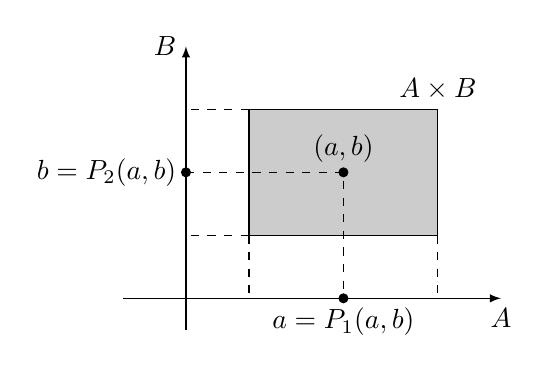
\begin{tikzpicture}[scale=.8]
			% Ejes
			\draw[-latex] (-1, 0) -- (5,0) node[below]{$A$};			
			\draw[-latex] (0, -.5) -- (0,4) node[left]{$B$};
			
			% Rectángulo
			\draw[fill=black!20] (1,1) rectangle (4, 3) node[above]{$A \times B$};
			
			% Puntos
			\draw[fill] (2.5,2) circle (2pt) node[above]{$(a,b)$};
			\draw[fill] (2.5,0) circle (2pt) node[below]{$a = P_1(a,b)$};
			\draw[fill] (0,2) circle (2pt) node[left]{$b = P_2(a,b)$};
			\draw[dashed] (1,1) -- (1,0);
			\draw[dashed] (1,1) -- (0,1);
			\draw[dashed] (0, 2) -- (2.5,2) -- (2.5,0);
			\draw[dashed] (4,1) -- (4,0);
			\draw[dashed] (1,3) -- (0,3);
		\end{tikzpicture}		
		\caption{Función proyección}
		\label{fig:funcion_proyeccion}
	\end{figure}
\end{itemize}

\begin{itemize}
	\item \textbf{Función canónica} \index{función!canónica}
	
	Sea $\sim$ o $\mathcal{R}$ una relación de equivalencia definida en el conjunto \textit{no vacío}
	$A$. Por el teorema fundamental de las relaciones de equivalencia, queda determinado
	el conjunto cociente $\dfrac{A}{\sim} = A/ \mathcal{R}$, cuyos elementos son las clases de equivalencia.
	
	\begin{fmd-definition}[Función canónica]
		Aplicación canónica es la función:
		\[ \varphi: A \rightarrow A / \mathcal{R} \]
		que asigna a cada elemento de $A$, su clase de equivalencia, es decir, tal que 
		\[ \varphi(x) = K_x = [x] \]
	\end{fmd-definition}
	
	Dos elementos equivalentes pertenecen a la misma clase y en consecuencia admiten la misma imagen, significa que la aplicación canónica \textbf{no es inyectiva}, salvo en caso de clases unitarias.
	
	Como cada clase es no vacía, ocurre que siempre \textbf{es sobreyectiva}:
	\[ \forall \, [u] \in A / \mathcal{R}, \exists \ x \in A / \varphi(x) = [u]  \]
	Vale la siguiente proposición:
	\[ a \equiv b \iff \varphi(a) = \varphi(b)\]
	En el caso de congruencia módulo 3, definida en $\mathbb{Z}$ es
	$\varphi: \mathbb{Z} \rightarrow \mathbb{Z}_3$ tal que $\varphi(x) = [u]$, siendo 
	$u$ el resto de la división de $x$ por 3.
\end{itemize}

\begin{fmd-example}
	Sea en $\R^2$ dos pares ordenados de reales que están relacionados si y sólo si tienen la misma primera
	componente. \[ \mathcal{R}: \, (a,b) \equiv (a', b') \iff a = a'\]
	La relación es de equivalencia, y el propósito es caracterizar
	la aplicación canónica.\vspace{1mm}
	
	Las clases de equivalencia son del tipo: $ K_{(a,b)} = \{ (x, y) / x = a \}$
	(rectas paralelas al eje de ordenadas) \vspace{1mm}
	
	Definir el conjunto cociente requiere un conjunto de índices, y al elegir un
	único elemento en cada clase, lo tomamos sobre el eje de abscisas, de modo que:
	\[ \R^2 / \mathcal{R} = \{ K_{(u,0)} / u \in \mathbb{R}\} \]
	Así la función canónica es $\phi: \mathbb{R}^2 \rightarrow \R^2 / \mathcal{R}$
	tal que $ \phi (a, b) = K_{(u, 0)} \mbox{ si } u = a $
	
	\begin{figure}[H]
		\centering
		\begin{tikzpicture}[scale=1.3]
			% Ejes x e y
			\draw[->] (-3,0) -- (4,0) node[below] {$x$};
			\draw[->] (0,-2.5) -- (0,2.5) node[right] {$y$};
			
			% Recta vertical en x = a
			\def\a{1.5}
			\draw[dashed, very thick, blue] (\a,0) -- (\a,2) node[above] {$K_{(a, 0)}$};
			\draw[dashed, very thick, blue] (\a,-2) -- (\a,-.5) node[above] {$x = a$};
			\draw[] (\a, 0) circle (1pt);
			
			% Serie de rectas verticales equidistantes
			\foreach \i in {-2,-1.5,...,3.5} {
				\draw[opacity=0.2] (\i,-2) -- (\i,2);
			}
		\end{tikzpicture}
		\caption*{La recta vertical por $x=a$ representa a la clase de equivalencia $K_{(a, 0)}$, de todos los puntos del plano con la misma primera componente $x=a$.}
	\end{figure}
	
\end{fmd-example}

\subsection{Composición de funciones} \label{sec:compos}
\index{composición!funciones} \index{funciones!composición}
Sean $f: A \rightarrow B$ y $g: B \rightarrow C$
\begin{figure}[H]
	\centering
	\begin{tikzpicture}[scale=.8]
		% Puntos
		\coordinate (a) at (0,0);
		\coordinate (b) at (6,0);
		\coordinate (c) at (12,0);
		
		% Circunferencias
		\draw[] (a) circle (2);
		\draw[] (b) circle (2);
		\draw[] (c) circle (2);
		\draw[dashed] (b) circle (3);
		\node at ($(a) + (-2, 1.5)$) {$A$};
		\node at ($(b) + (-2, 1.5)$) {$B$};
		\node at ($(b) + (-2, 3)$) {$B'$};
		\node at ($(c) + (-2, 1.5)$) {$C$};
		
		% Centros
		\draw[fill] (a) circle (2pt) node[below]{$x$};
		\draw[fill] (b) circle (2pt) node[below]{$f(x)$};
		\draw[fill] (c) circle (2pt) node[above, yshift=8] {$(g \circ f)(x)$};
		
		% Flechas
		\draw[-latex, blue, thick] (a) to [bend left = 15] (b);
		\draw[-latex, blue, thick] (b) to [bend left = 15] (c);
		\draw[-latex, blue, thick] (a) to [bend right = 25] (c);
	\end{tikzpicture}
	\caption{Composición de funciones}
	\label{fig:compos1}
\end{figure}
El codominio de $f$ es dominio de $g$, pero es suficiente que el codominio de la
primera sea parte del dominio de la segunda: $B \subset B'$. En la fig. \ref{fig:compos1} se ve gráficamente esta afirmación.

\begin{fmd-definition}[Composición de funciones]
	La \gls{composicion} entre $f: A \rightarrow B$ y $g:B \rightarrow C$ es la
	función $g \circ f : A \rightarrow C$, tal que:
	$ (g \circ f)(x) = g\left[ f(x) \right] \ \forall x \in A$
\end{fmd-definition}

\begin{fmd-example}[Composición de funciones discretas]
	Sean $A = \{ 1, 2, 3 \}$, $B = \{ a, b, c, d \}$, $C = \{ 5, 6 \}$ y las funciones
	$f: A \rightarrow B$ y $g: B \rightarrow C$ definidas así:
	\[ f: \{(1, a), (2, b), (3, d)\}; \quad g = \{ (a, 5), (b, 5), (c, 5), (d, 6) \} \]
	Resulta: $g \circ f = \{(1,5), (2, 5), (3, 6) \}$. Ver figura.
	
	\begin{figure}[H]
		\centering
		\begin{tikzpicture}[scale=.8]
			% Centros
			\coordinate (a) at (0,0);
			\coordinate (b) at (6,0);
			\coordinate (c) at (12,0);
			
			% Circunferencias
			\draw[] (a) circle (2);
			\draw[] (b) circle (2);
			\draw[] (c) circle (2);
			
			\node at ($(a) + (-1.5,2)$) {$A$};
			\node at ($(b) + (-1.5,2)$) {$B$};
			\node at ($(c) + (-1.5,2)$) {$C$};
			
			% Elementos
			\coordinate (A1) at ($(a) + (-.5, 1)$);
			\coordinate (A2) at ($(a) + (-.5, 0)$);
			\coordinate (A3) at ($(a) + (-.5, -1)$);
			
			\draw[fill] (A1) circle (2pt) node[left]{$1$};
			\draw[fill] (A2) circle (2pt) node[left]{$2$};
			\draw[fill] (A3) circle (2pt) node[left]{$3$};
			
			\coordinate (B1) at ($(b) + (0, 1.5)$);
			\coordinate (B2) at ($(b) + (0, .5)$);
			\coordinate (B3) at ($(b) + (0, -.5)$);
			\coordinate (B4) at ($(b) + (0, -1.5)$);
			
			\draw[fill] (B1) circle (2pt) node[above]{$a$};
			\draw[fill] (B2) circle (2pt) node[above]{$b$};
			\draw[fill] (B3) circle (2pt) node[above]{$c$};
			\draw[fill] (B4) circle (2pt) node[above]{$d$};
			
			\coordinate (C1) at ($(c) + (0, 1)$);
			\coordinate (C2) at ($(c) + (0, -1)$);
			
			\draw[fill] (C1) circle (2pt) node[right] {$5$};
			\draw[fill] (C2) circle (2pt) node[right] {$6$};
			
			% Flechas
			\draw[-latex, blue, thick] (A1) to [bend left = 15] (B1);
			\draw[-latex, blue, thick] (A2) to [bend left = 15] (B2);
			\draw[-latex, blue, thick] (A3) to [bend right = 15] (B4);
			
			\draw[-latex, blue, thick] (B1) to [bend left = 15] (C1);
			\draw[-latex, blue, thick] (B2) to [bend right = 15] (C1);
			\draw[-latex, blue, thick] (B3) to [bend right = 15] (C1);
			\draw[-latex, blue, thick] (B4) to [bend right = 15] (C2);
		\end{tikzpicture}
		\label{fig:compos2}
	\end{figure}
	Nótese que no coexisten $g \circ f$ y $f \circ g$ ya que, en este caso, el codominio
	de $g$ es $C$ y el dominio de $f$ es $A$. Ambas composiciones existen si $C \subset A$.
\end{fmd-example}

\begin{fmd-example}[Composición de funciones continuas] \label{ex:compos}
	Sean: \[ \begin{cases}
		f: \mathbb{R} \rightarrow \mathbb{R} & \mbox{tal que } f(x) = 2x \\
		g: \mathbb{R} \rightarrow \mathbb{R} & \mbox{tal que } g(x) = x^2
	\end{cases}
	\]
	\begin{enumerate}
		\item $g \circ f: \mathbb{R} \rightarrow \mathbb{R}$ es:
		$ (g \circ f)(x) = g\left[ f(x) \right] = g(2x) = (2x)^2 = 4x^2$
		\item $f \circ g: \mathbb{R} \rightarrow \mathbb{R}$ es:
		$ \left( f \circ g \right)(x) = f\left[g(x)\right] = f(x^2) = 2 x^2 $
	\end{enumerate}
	Ambas funciones compuestas, a pesar de tener el mismo dominio y codominio, son
	distintas, por diferir en la ley de asignación.
\end{fmd-example}

\begin{definition}[Funciones iguales] \index{funciones!iguales}
	Dos funciones $f:A \rightarrow B$ y $g: A \rightarrow B$ son iguales si y sólo si
	para todo $x$ de $A$ se verifica $f(x) = g(x)$
\end{definition}\vspace{2mm}
Con relación al ejemplo \ref{ex:compos} $g \circ f \ne f \circ g$.

\subsubsection{Asociatividad de la composición} \label{sec:asocom}
Si $f: A \rightarrow B$, $g: B \rightarrow C$ y $h: C \rightarrow D$, entonces:
$\left( h \circ g \right) \circ f = h \circ \left( g \circ f \right)$
\begin{figure}[H]
	\centering
	\begin{tikzpicture}[scale=.8]
		% Puntos
		\coordinate (a) at (0,0);
		\coordinate (b) at (5,0);
		\coordinate (c) at (10,0);
		\coordinate (d) at (15,0);
		
		% Circunferencias
		\draw[] (a) circle (2);
		\draw[] (b) circle (2);
		\draw[] (c) circle (2);
		\draw[] (d) circle (2);
		
		\node at ($(a) + (-2, 1.5)$) {$A$};
		\node at ($(b) + (-2, 1.5)$) {$B$};
		\node at ($(c) + (-1.5, 2)$) {$C$};
		\node at ($(d) + (-2, 1.5)$) {$D$};
		
		% Centros
		\draw[fill] (a) circle (2pt) node[below]{$x$};
		\draw[fill] (b) circle (2pt) node[below left]{$f(x)$};
		\draw[fill] (c) circle (2pt) node[below] {$g[f(x)]$};
		\draw[fill] (d) circle (2pt) node[above] {$h\{g[f(x)]\}$};
		
		% Flechas
		\draw[-latex, blue, thick] (a) to [bend left = 15] (b);
		\draw[-latex, blue, thick] (b) to [bend left = 15] (c);
		\draw[-latex, blue, thick] (c) to [bend left = 10] (d);
		\draw[-latex, blue, thick] (a) to [bend left = 50] (c);
		\draw[-latex, blue, thick] (b) to [bend right = 50] (d);
		
		\node at (4, 2.8) {$g \circ f$};
		\node at (10, -2.8) {$h \circ g$};
	\end{tikzpicture}
	\caption{Asociatividad de la composición}
	\label{fig:compos3}
\end{figure}

En efecto, $\forall x \in A$:
\[\begin{cases}
	\left( (h \circ g) \circ f \right)(x) &= (h \circ g)\left(f(x)\right) = h \{ g[f(x)]\}\\
	\left( h \circ (g \circ f) \right)(x) &= h \left( (g \circ f)(x)\right) = h \{ g[f(x)]\}
\end{cases} \]
De donde resulta la igualdad buscada. Ver fig. \ref{fig:compos3}.


\subsubsection{Composición de funciones inyectivas} \label{sec:cominy}
\vspace{1em}
\begin{fmd-proposition}
	Si $f: A \rightarrow B$ y $g: B \rightarrow C$ son inyectivas, entonces $g \circ f: 
	A \rightarrow C$ es inyectiva.
\end{fmd-proposition}

\begin{fmd-proof}
	Debemos probar: H) $\forall \, x', x'' \in A$ con $(g \circ f)(x') = (g \circ f)(x'')$, 
	entonces T) $x' = x''$
	
	Por hipótesis y por definición de composición:
	\[ g[f(x')] = g[f(x'')] \]
	por ser $g$ inyectiva:
	\[ f(x') = f(x'')\]
	por ser $f$ inyectiva:
	\[x' = x'' \]
	\emph{La composición de funciones inyectivas es inyectiva}.
\end{fmd-proof}


\subsubsection{Composición de funciones sobreyectivas} \label{sec:comsob}
\vspace{1em}
\begin{fmd-proposition}
	Si $f: A \rightarrow B$ y $g: B \rightarrow C$ son sobreyectivas, entonces $g \circ f: 
	A \rightarrow C$ es sobreyectiva.
\end{fmd-proposition}
\begin{fmd-proof}
	Hay que probar que $\forall \, z \in C \, \exists \, x \in A$ tal que
	$(g \circ f)(x) = z$.\vspace{2mm}
	
	Por ser $g$ sobreyectiva:
	$\forall \, z \in C, \, \exists \, y \in B / g(y) = z$
	
	Ahora bien, dado que $y \in B$, por ser $f$ sobreyectiva
	$\exists \, x \in A / f(x) = y$
	
	De aquí se deduce que:
	\[g[f(x)] = g(y) = z\]
	
	\emph{La composición de funciones sobreyectivas es sobreyectiva}.
\end{fmd-proof}

Se sigue de los casos anteriores que, si $f: A \rightarrow B$ y $g: B \rightarrow C$ son biyectivas, entonces $g \circ f: 
A \rightarrow C$ es biyectiva.

\begin{fmd-example}
	Demostrar que si $f: A \rightarrow B$ y $g: B \rightarrow C$ son tales que
	$g \circ f: A \rightarrow C$ es inyectiva, entonces $f$ es inyectiva.\vspace{-2mm}
	
	\begin{proof}
		Sean $x', x'' \in A$ tales que $f(x') = f(x'')$, la imagen de este elemento de $B$
		por $g$, es:
		\[ g[f(x')] = g[f(x'')] \]
		ya que cada elemento del dominio $B$ tiene imagen única en $C$, por definición de
		función. Por definición de composición
		\[ (g \circ f)(x') = (g \circ f)(x'') \]
		y por ser $g \circ f$ inyectiva, resulta $x'=x''$, en consecuencia $f$ es
		inyectiva.
	\end{proof}
	
	Análogamente se demuestra que si la composición de dos aplicaciones es sobreyectiva,
	la segunda es sobreyectiva.
\end{fmd-example}

\subsection{Funciones inversas} \label{sec:finversas} \index{función!inversa}
Cabe preguntarse si, para la función $f: A \rightarrow B$, la relación inversa
es una función. En general la respuesta es negativa, como se ve a través del ejemplo 2,
diapositiva \ref{frame:ejm2}, donde $A = \{-1,0,1,2\}$, $B=\{0,1,2,3,4\}$ y $f(x) =x^2$
\[ f = \{ (-1,1), (0,0), (1,1), (2,4) \} \]
la inversa de esta relación es el subconjunto $B \times A$
\[ \{ (1,-1), (0,0), (1,1), (4,2) \} \]
se ve que esta relación no es una función de $B$ en $A$, pues los elementos 2
y 3 del eventual dominio carecen de imágenes en $A$ y además no se cumple la
condición de unicidad, ya que 1 tiene dos correspondientes en $A$.

Sea, en cambio, el siguiente caso $A = \{1,2,3\}$, $B=\{a,b,c\}$ y 
$f(x) =\{(1, a), (2, c), (3,b) \}$. La relación inversa es:
\[ g = \{ (a,1), (b,3), (c,2) \} \]
es claramente una función de $B$ en $A$, llamada \gls{funcioninversa} de $f$. La composición
\[ g \circ f = \{ (1,1),(2,2),(3,3) \} = i_A \]
en donde $g$ es la \textit{inversa izquierda} de $f$
y \[ f \circ g = \{ (a, a), (b,b), (c,c) \} = i_B\]
En este caso $g$ es la \textit{inversa derecha} de $f$ \vspace{2mm}

\begin{mdframed}[backgroundcolor=gray!20, linecolor=black, linewidth=1pt]
	La función $f: A \rightarrow B$ admite inversa si y sólo si existe
	$g: B \rightarrow A$ tal que $g \circ f = i_A$ y $f \circ g = i_B$
\end{mdframed}

\begin{fmd-example}[Función inversa]
	La función $f: \mathbb{R} \rightarrow \mathbb{R}$ definida por $f(x) = x + 2$ admite
	inversa $g: \mathbb{R} \rightarrow \mathbb{R}$ tal que $g(x) = x - 2$, pues
	\[
	\begin{cases}
		(g \circ f)(x) &= g[f(x)] = g(x+2) = x + 2 -2 = x = i_\mathbf{R}(x)\\
		(f \circ g)(x) &= f[g(x)] = f(x-2) = x - 2 + 2 = x = i_\mathbf{R}(x)\\
	\end{cases}	
	\]
	La representación cartesiana de dos funciones inversas conduce a gráficos simétricos
	respecto de la recta a $45\unit{\degree}$.
	
	\begin{figure}[H]
		\centering
		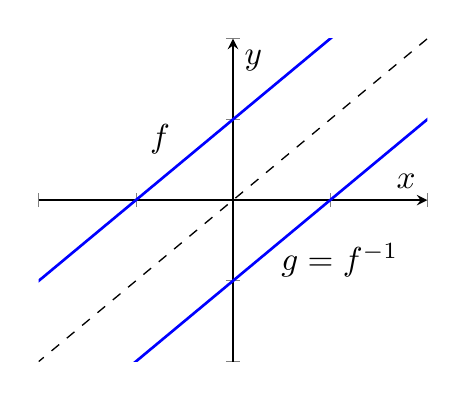
\begin{tikzpicture}[scale=1.2]
			\begin{axis}[axis lines=middle, xmin=-4, xmax=4,
				ymin=-4, ymax=4, xticklabels={}, yticklabels={},
				xlabel={$x$}, ylabel={$y$}, scale=.6]
				\addplot[dashed] {x};
				\addplot[blue, thick] {x - 2} node[below]{$g$};
				\addplot[blue, thick] {x + 2};
				\node at (axis cs:-1.5,1.5) {$f$};
				\node at (axis cs:2.2,-1.5) {$g=f^{-1}$};
			\end{axis}
		\end{tikzpicture}
	\end{figure}
\end{fmd-example}

\begin{fmd-theorem}
	Una función admite inversa si y sólo si es biyectiva.
\end{fmd-theorem}

\begin{enumerate}
	\item Si una función admite inversa, entonces es biyectiva.
	\begin{itemize}
		\item[H)] $f: A\rightarrow B$ es tal que $\exists \, g: B \rightarrow A$
		siendo $g \circ f = i_A$ y $f \circ g = i_B$
		\item[T)] $f$ es biyectiva.
	\end{itemize}
	\begin{proof}
		En dos partes.
		\begin{enumerate}[label=\alph*)]
			\item Inyectividad de $f$
			
			Sean $x', x'' \in A / f(x') = f(x'') \in B$.
			
			La imagen por $g$ es $g[f(x')] = g[f(x'')] $, o,
			$(g \circ f)(x') = (g \circ f)(x'')$
			
			siendo $g \circ f = i_A$, se tiene $i_A(x') = i_A(x'')$ o, lo que es lo mismo:
			$x' = x''$.
			
			Por tanto $f$ es 1-1.

		\item $f$ es sobreyectiva
		
		Según definición, hay que probar $\forall \, y \in B, \exists \, x \in A /
		f(x) = y$\vspace{2mm}
		
		Sea $y \in B$, entonces $y = i_B(y)$, y como $i_B = f \circ g$, se tiene:
		\[ y = (f \circ f)(y), \mbox{ es decir, } y= f[g(x)] \]
		por tanto, a expensas de $y \in B$, hemos determinado $x = g(y)$ en $A$,
		tal que $f(x) = y$
	\end{enumerate}
\end{proof}
Siendo $f$ inyectiva y sobreyectiva resulta biyectiva.


	\item Si una función es biyectiva, entonces admite inversa.
	
	\begin{itemize}
		\item[H)] $f: A \rightarrow B$ es biyectiva.
		\item[T)] $\exists \, g: B \rightarrow A$ tal que $g \circ f = i_A$ y
		$f \circ g = i_B$
	\end{itemize}
	
	\begin{proof}
		Necesitamos proceder en tres etapas.
		
		\begin{enumerate}[label=\textbf{\alph*)}]
			\item Definimos
			$g: B \rightarrow A \mbox{ mediante } g(y)= x \mbox{ si } f(x) = y
			\quad (1)$
			
			que satisface la definición de función, pues:
			\begin{enumerate}[label=\roman*), ref=\roman*]
				\item Todo $y \in B$ proviene de algún $x \in A$
				\item La $x$ asociada a $y$ es única, por ser $f$ inyectiva.
				
				En efecto, si $x$ y $x'$ fueran antecedentes distintos de $y$ por $f$
				se tendría $x \ne x'$ y $f(x) = f(x') = y$, lo que es absurdo por la
				inyectividad de $f$.
			\end{enumerate}
		\item Hay que probar que $g \circ f = i_A$.
		
		$\forall x \in A$, se tiene, por definición de composición, por (1), y
		por definición de identidad en $A$:
		\[ (g \circ  f)(x) = g[f(x)] = g(y) = x = i_A(x)\]
		Entonces, por definición de funciones iguales:
		\[ g \circ f = i_A \]

		\item Finalmente, demostramos que $f \circ g = i_B$
		
		Como $f \circ g: B \rightarrow B \ \forall \, y \in B$, tenemos, por definición
		de composición, por (1) y por identidad en $B$.
		
		\[ (f \circ g)(y) = f[g(y)] = f(x) = y = i_B(y) \]
		Con lo cual:
		\[ f \circ g = i_B \]
	\end{enumerate}
\end{proof}
\end{enumerate}

\begin{mdframed}[backgroundcolor=gray!20, linecolor=black, linewidth=1pt,
	frametitle={Consecuencia}]
	Si $f: A \rightarrow B$ es biyectiva, entonces la función $g:B \rightarrow A$ a 
	que se refiere el teorema anterior, es única y, además, biyectiva.
\end{mdframed}
\begin{proof}
	Si existieran dos funciones $g$ y $g'$ se tendría:
	\[ g' = g' \circ i_B = g' \circ (f \circ g) = (g' \circ f) \circ g = 
	i_A \circ g = g \]
	
	Por otra parte, como una función que admite inversa es biyectiva, se tiene 
	que $g: B \rightarrow A$ es tal que $\exists \, f: A \rightarrow B$, siendo
	$f \circ g = i_B$ y $g \circ f = i_A$. En consecuencia, $g$ es biyectiva
\end{proof}

La función $g$ se llama inversa y se denota por $f^{-1}$.

\begin{fmd-example}
	Probar que $f: \mathbb{R} \rightarrow (-1, 1)$ definida por 
	$f(x) = \dfrac{x}{1 + |x|}$ admite inversa.
	
	\begin{enumerate}[label=\textbf{\alph*)}]
		\item $f$ es inyectiva
		
		Sean $x', x'' \in A / f(x') = f(x'')$
		\[ \frac{x'}{1 + |x'|} = \frac{x''}{1 + |x''|} \implies x' + x'|x''| = 
		x'' + x'' |x'| \implies x' = x'' \]
		O sea, $f$ es 1-1.
		\item $f$ es sobreyectiva
		
		Sea $y \in (-1, 1)$. Si $\exists \, x \in \mathbb{R} / f(x) = y$, entonces 
		$\dfrac{x}{1 + |x|} = y$, notar que $x$ y $y$ tienen signos iguales, $\mathrm{sg}(x) = \mathrm{sg}(y)$.
		
		Operando (siendo $|y| < 1$):
		\[ x = y + y|x| \rightarrow x = y + y \, x \, \mathrm{sg}(x) \rightarrow
		x = y + x \, y \, \mathrm{sg}(y) \rightarrow x - x \, y \, \mathrm{sg}(y) = y \]
		\[ \rightarrow x(1 - |y|) = y \rightarrow x = \frac{y}{1 - |y|}\]
	
		de donde: $\forall \, y \in (-1, 1), \exists \, x = \dfrac{y}{1 - |y|}$ tal que:
		\[ f(x) = f \left( \frac{y}{1 - |y|} \right) = \frac{\dfrac{y}{1-|y|}}{1 - 
			\left| \dfrac{y}{1 - |y|} \right|} = \frac{\dfrac{y}{1 - |y|}}{1 - \dfrac{|y|}
			{1 - |y|}} = y \]
		lo que prueba que $f$ es sobreyectiva.
\end{enumerate}
	
	Por a) y b) resulta que $f$ es biyectiva y en consecuencia admite inversa. La 
	inversa es: \[ f^{-1}: (-1,1) \rightarrow \mathbb{R} / f^{-1}(x) = \dfrac{x}{1 - |x|}\]
	
	Se puede verificar que $g \circ f = i_\mathbb{R}$ y que $f \circ g = i_{(-1,1)}$.
\end{fmd-example}

\begin{fmd-example}
	La función $f: A \rightarrow B$ es inyectiva si y sólo si existe $g: B \rightarrow A$
	tal que $g \circ f = i_A$.
	
	\begin{itemize}
		\item[H)] $f: A \rightarrow B$ es 1-1;
		\item[T)] $\exists \, g: B \rightarrow A / g \circ f = i_A$
	\end{itemize}\vspace{3mm}
	
	La función $f$ no es necesariamente sobreyectiva. Nos apoyamos en el diagrama de la figura siguiente:
	\begin{figure}[H]
		\centering
		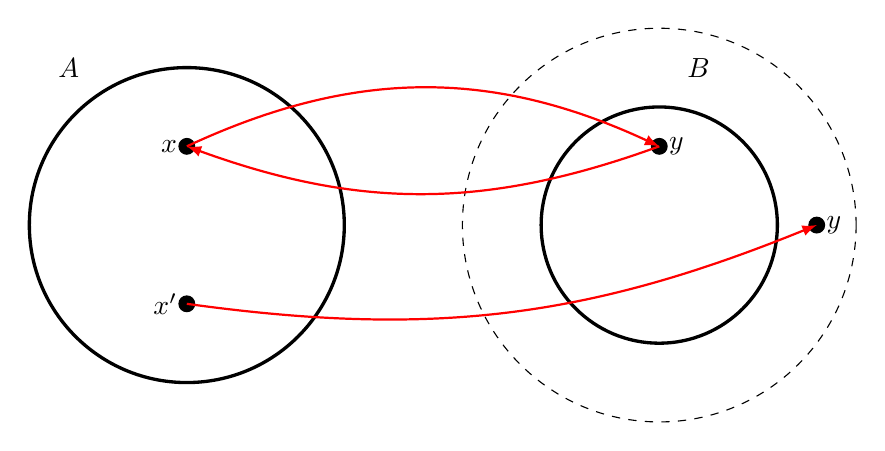
\begin{tikzpicture}[scale=1]
			% Coordenadas de puntos
			\coordinate (x1) at (0,1);
			\coordinate (x2) at (0,-1);
			
			\coordinate (y1) at (6,1);
			\coordinate (y2) at (8,0);
			
			% Circunferencias
			\node at (-1.5, 2) {$A$};
			\node at (6.5, 2) {$B$};
			\draw[very thick] (0,0) circle (2);
			\draw[very thick] (6,0) circle (1.5);
			\draw[dashed] (6,0) circle (2.5);
			
			% Puntos
			\draw[fill] (x1) circle (1mm) node[left] {$x$};
			\draw[fill] (x2) circle (1mm) node[left] {$x'$};
			
			\draw[fill] (y1) circle (1mm) node[right] {$y$};
			\draw[fill] (y2) circle (1mm) node[right] {$y$};
			
			% flechas
			\draw[red, thick, -latex] (x1) to [bend left = 25] (y1);
			\draw[red, thick, -latex] (x2) to [bend right = 15] (y2);
			\draw[red, thick, -latex] (y1) to [bend left = 20] (x1);
		\end{tikzpicture}
	\end{figure}
	
	\begin{proof}
		Definimos una función $g: B \rightarrow A$:
		\[ g(y) \begin{cases}
			x & \mbox{si } f(x) = y\\
			x' & \mbox{(cualquier elemento fijo de $A$) si } \nexists \, x \in A 
			/ f(x) = y
		\end{cases} \]
		De este modo, todo elemento de $B$ tiene su correspondiente en $A$, y es único por
		ser $f$ inyectiva. Ahora bien:
		
		\[ (g \circ f)(x) = g[f(x)] = g(y) = x = i_A(x) \]
		luego: \[ g \circ f = i_A \]
	\end{proof}
	
	\begin{enumerate}
		\setcounter{enumi}{1}
		\item \begin{itemize}
			\item[H)] $f: A \rightarrow B$ es tal que existe $g:B \rightarrow A$ de modo
			que $g \circ f = i_A$;
			\item[T)] $f$ es inyectiva.
		\end{itemize}\vspace{3mm}
		\begin{proof}
			Sean $x', x'' \in A / f(x') = f(x'')$, entonces
			\[ g[f(x')] = g[f(x'')] \mbox{o, lo que es lo mismo } (g \circ f)(x') = (g \circ f)(x'') \]
			por hipótesis: \[\mbox{Si } i_A(x') = i_A(x'') \mbox{ entonces } x' = x''\]
			
			en consecuencia $f$ es 1-1\
		\end{proof}
	\end{enumerate}
\end{fmd-example}

\textbf{Resumen de funciones inversas}
\begin{fmd-definition}[Función inversa]
	Sea $f$ una función biyectiva con dominio $X$ y rango $Y$. La \textbf{inversa}
	de $f$ es la función $f^{-1}$ cuyo dominio es $Y$ y rango es $X$, para los cuales
	
	\[ f \circ f^{-1} = f[f^{-1}(x)] = x \quad \forall x \in Y \]
	y \[ f^{-1} \circ f = f^{-1}[f(x)] = x  \quad \forall x \in X\]
\end{fmd-definition}

\underline{\textbf{Propiedades}}:

		\begin{enumerate}[label=\roman*)]
			\item Dominio $f^{-1}$ = rango $f$;
			\item Rango $f^{-1}$ = dominio $f$;
			\item $y = f(x)$ equivale a $x = f^{-1}(y)$;

			\setcounter{enumi}{3}
			\item $f^{-1}$ es biyectiva;
			\item $(f^{-1})^{-1} = f$;
			\item La inversa de $f$ es única.
		\end{enumerate}


\subsection{Imágenes de subconjuntos del dominio} \label{sec:imasub}
Sean $f : X \rightarrow Y$ y $A \subset X$ \index{imagen}
\begin{fmd-definition}[Imagen de subconjuntos]
	Imagen del subconjunto $A \subset X$ es el conjunto cuyos elementos son las
	imágenes de los elementos de $A$.
\end{fmd-definition}

\begin{figure}[H]
	\centering
	\begin{tikzpicture}[scale=1]
		% Centros
		\coordinate (a) at (0,0);
		\coordinate (b) at (5,0);
		
		% Circunferencias
		\draw[] (a) circle (2);
		\draw[] (b) circle (2);
		
		\node at ($(a) + (-1.5,2)$) {$X$};
		\node at ($(b) + (-1.5,2)$) {$Y$};
		
		% Elipses
		\draw[fill=black!20] (a) ellipse (1 and .6);
		\draw[fill=black!20] (b) ellipse (1 and .6);
		
		\node at ($(a) + (-1, .7)$) {$A$};
		\node[above right] at ($(b) + (3, -.5)$) {$f(A)$: ``imagen de $A$''};
		
		% Flechas
		\draw[blue, thick, -latex] (a) to [bend left = 15] ($(b) + (-1, .2)$);
		\draw[blue, thick, -latex] ($(b) + (.5,-.1)$) to [bend right = 10]
		($(b) + (3, -.5)$);
	\end{tikzpicture}
	\caption{Imagen de subconjuntos}
	\label{fig:imagenes}
\end{figure}
\[ f(A) = \{ f(x) / x \in A \} \mbox{ o bien } f(A) = \{y \in Y / \mbox{ existe } \, 
x \in A \mbox{ y } f(x) = y \} \]
De acuerdo con la definición: $y \in f(A) \mbox{ si y solo si existe } x \in A / y = f(x)$

Si $A = X$, entonces $f(X)$ es la imagen del dominio por $f$. Además
$f(\emptyset) = \emptyset$. $f$ es sobreyectiva si y sólo si $f(X) = Y$.

\subsubsection{Propiedades de la imagen}
Sean $f: X \rightarrow Y$ y $A$ y $B$ subconjuntos del dominio.
\begin{enumerate}[label=\textbf{\alph*)}]
	\item Si un subconjunto del dominio es parte de otro, entonces la misma relación
	vale para sus imágenes.
	\[ f: X \rightarrow Y, A \subset B, B \subset X \mbox{ y } A \subset B \mbox{ entonces }
	f(A) \subset f(B)\]
	En efecto, sea
	\[ z \in f(A) \rightarrow \mbox{ hay algún } \, x \in A / f(x) = z \rightarrow \mbox{ existe } \, x
	\in B / f(x) = z \rightarrow z \in f(B) \]
\end{enumerate}


\begin{enumerate}[label=\textbf{\alph*)}]
	\setcounter{enumi}{1}
	\item La imagen de la unión de dos subconjuntos del dominio, es igual a la 
	unión de sus imágenes.
	\[ f: X \rightarrow Y , A \subset X \land B \subset X \implies f\left( A 
	\cup B \right) = f(A) \cup f(B) \]
	\begin{figure}[H]
		\centering
		\begin{tikzpicture}[scale=1]
			% Centros
			\coordinate (x) at (0,0);
			\coordinate (a) at (-.5,.5);
			\coordinate (b) at (.5,-.5);
			
			\coordinate (y) at (5, 0);
			\coordinate (fa) at (4.5,.5);
			\coordinate (fb) at (5.5,-.5);
			
			% Circunferencias
			\draw[thick] (x) circle (2);
			\filldraw[pattern=north east lines] (a) circle (1);
			\filldraw[pattern=north west lines] (b) circle (1);
			\draw[thick] (y) circle (2);
			\filldraw[pattern=north east lines] (fa) circle (1);
			\filldraw[pattern=north west lines] (fb) circle (1);
			
			\node at ($(x) + (-2,1.5)$) {$X$};
			\node at ($(y) + (-2,1.5)$) {$Y$};
			\node at ($(a) + (-1,-1)$) {$A$};
			\node at ($(b) + (-1,-1)$) {$B$};
			\node at ($(fa) + (1,1)$) {$f(A)$};
			\node at ($(fb) + (-1,-1)$) {$f(B)$};
			
			% Flechas
			\draw[-latex, blue, thick] (a) to [bend left = 10] (fa);
			\draw[-latex, blue, thick] (b) to [bend right = 15] (fb);
		\end{tikzpicture}
		\caption{Imagen de la unión de dos subconjuntos.}
		\label{fig:imagenes2}
	\end{figure}
\end{enumerate}

\begin{enumerate}[label=\textbf{\alph*)}]
	\setcounter{enumi}{2}
	\item La imagen de la intersección de dos subconjuntos del dominio está incluida
	en la intersección de sus imágenes.
	\[ \mbox{Si } f: X \rightarrow Y, A \subset X \mbox{ y } B \subset X \mbox{ entonces } f\left( 
	A \cap B \right) \subset f(A) \cap f(B) \]
	
	El siguiente ejemplo prueba que no es válida la inclusión en el otro sentido.
	
	Sean $f: \mathbb{Z} \rightarrow \mathbb{N} / f(x) = x^2$ y los subconjuntos de 
	$\mathbb{Z}$
	\[ A = \{ -2, -3, 4 \} \mbox{ y } B = \{ 2, 3, 4, 5 \} \]
	Se tiene $A \cap B = \{ 4 \}$, $f\left( A \cap B \right) = \{16\}$, $f(A) \cap f(B)
	= \{ 4, 9, 16\}$
	
	Resulta:
	\[ f\left( A \cap B \right) \not \subset f(A) \cap f(B) \]
\end{enumerate}

\subsection{Imágenes inversas de subconjuntos del codominio} \label{sec:invcon}
\index{imagen!inversa}
Sean $f: X \rightarrow Y$ y $A \subset Y$.

\begin{fmd-definition}[Preimagen] \label{def:preimagen} \index{preimagen}
	Imagen inversa o preimagen del subconjunto $A \subset Y$, es el conjunto de los
	elementos del dominio cuyas imágenes pertenecen a $A$.
	
	\begin{figure}[H]
		\centering
		\begin{tikzpicture}[scale=1]
			% Centros
			\coordinate (x) at (0,0);
			\coordinate (y) at (5, 0);
			
			% Circunferencias
			\draw[] (x) circle (2);
			\draw[] (y) circle (2);
			\filldraw[pattern=north east lines] (x) circle (1);
			\filldraw[pattern=north west lines] (y) circle (1);
			
			\node at ($(x) + (-2,1.5)$) {$X$};
			\node at ($(y) + (-2,1.5)$) {$Y$};
			\node at ($(x) + (0,-1.5)$) {$f^{-1}(A)$};
			\node at ($(y) + (-1,-1)$) {$A$};
			
			% Flechas
			\draw[latex-, blue, thick] (x) to [bend left = 20] (y);
		\end{tikzpicture}
		\caption{Definición de preimagen}
		\label{fig:preimagen}
	\end{figure}
	\[ f^{-1}(A) = \{ x \in X / f(x) \in A \} \]
	Es claro que: $ x \in f^{-1}(A)$ si, y solo si $f(x) \in A $, en palabras, un elemento del dominio pertenece a la preimagen de $A$ si y sólo si su imagen pertenece a $A$.
\end{fmd-definition}

\begin{fmd-example}[Preimagen]
	Sea $f: \mathbb{R} \rightarrow \mathbb{R} / f(x) = x^2$. Determinamos las preimágenes
	de los siguientes subconjuntos del codominio
	\[ (-\infty, -1], (-1, 1], (-1, 1), [4,9] \]
	\begin{enumerate}[label=\roman*)]
		\item $f^{-1} (-\infty, -1] = \{ x \in \mathbb{R} / f(x) \in (-\infty, -1] \}$
		
		Ahora bien \[ f(x) \in (-\infty, -1) \iff x^2 \le -1 \iff x \in \varnothing \]
		Resulta
		\[ f^{-1} (-\infty, -1] = \varnothing \]
	\end{enumerate}
	
	
	\begin{enumerate}[label=\roman*)]
		\setcounter{enumi}{1}
		\item En el segundo caso:
		\[ x \in f^{-1}(-1, 1] \rightarrow f(x) \in (-1, 1] \rightarrow x^2 \in (-1, 1]
		\rightarrow -1 < x \le 1\]
		\[ \rightarrow x^2 \le 1 \rightarrow |x|^2 \le 1 \rightarrow -1 \le x \le 1
		\rightarrow x \in [-1, 1] \]
		Entonces $f^{-1}(-1, 1] = [-1, 1]$
		\item Se tiene \[ x \in f^{-1}(-1,1) \rightarrow f(x) \in (-1,1) \rightarrow
		x^2 \in (-1, 1) \rightarrow x^2 < 1 \]
		\[ \rightarrow |x| < 1  \rightarrow -1 < x < 1 \rightarrow x \in (-1, 1)\]
		Luego $f^{-1} (-1,1) = (-1,1)$
	\end{enumerate}
	
	\begin{enumerate}[label=\roman*)]
		\setcounter{enumi}{3}
		\item Finalmente
		\[ x \in f^{-1}[4,9] \rightarrow f(x) \in [4,9] \rightarrow x^2 \in [4,9]
		\rightarrow 4 \le x^2 \le 9 \]
		\[ \rightarrow x^2 \ge 4 \land x^2 \le 9 \rightarrow |x| \ge 2 \land |x|\le 3
		\]
		\[ \rightarrow x \in [-3, -2] \vee x \in [2, 3] \rightarrow x \in [-3,-2] 
		\cup [2,3] \]
		Entonces: \[ f^{-1}[4,9] = [-3, -2] \cup [2,3] \]
	\end{enumerate}
\end{fmd-example}

\subsubsection{Propiedades de la preimagen}
Sean $f:X \rightarrow Y$ y los subconjuntos $A \subset Y$, $B \subset Y$.
\begin{enumerate}[label=\textbf{\alph*)}]
	\item La preimagen de la unión es la unión de las preimágenes.
	\[ f^{-1} \left( A \cup B \right) = f^{-1}(A) \cup f^{-1}(B) \]
	\begin{figure}[H]
		\centering
		\begin{tikzpicture}[scale=1]
			% Centros
			\coordinate (x) at (0,0);
			\coordinate (a) at (-.5,.5);
			\coordinate (b) at (.5,-.5);
			
			\coordinate (y) at (5, 0);
			\coordinate (fa) at (4.5,.5);
			\coordinate (fb) at (5.5,-.5);
			
			% Circunferencias
			\draw[thick] (x) circle (2);
			\filldraw[pattern=north east lines] (a) circle (.8);
			\filldraw[pattern=north west lines] (b) circle (.8);
			\draw[thick] (y) circle (2);
			\filldraw[pattern=north east lines] (fa) circle (1);
			\filldraw[pattern=north west lines] (fb) circle (1);
			
			\node at ($(x) + (-2,1.5)$) {$X$};
			\node at ($(y) + (-2,1.5)$) {$Y$};
			\node at ($(a) + (1,1)$) {$f^{-1}(A)$};
			\node at ($(b) + (-1,-1)$) {$f^{-1}(B)$};
			\node at ($(fa) + (1,1)$) {$A$};
			\node at ($(fb) + (-1,-1)$) {$B$};
			
			% Flechas
			\draw[latex-, blue, thick] (a) to [bend left = 10] (fa);
			\draw[latex-, blue, thick] (b) to [bend right = 15] (fb);
		\end{tikzpicture}
		\caption{Preimagen de la unión $A \cup B$.}
		\label{fig:imagenes3}
	\end{figure}
	\[ x \in f^{-1}\left( A \cup B \right) \rightarrow f(x) \in A \cup B \rightarrow
	f(x) \in A \mbox{ o } f(x) \in B \]
	\[ \rightarrow x \in f^{-1}(A) \mbox{ o } x \in f^{-1}(B) \rightarrow x \in f^{-1}
	(A) \cup f^{-1} (B)\]
\end{enumerate}

\begin{enumerate}[label=\textbf{\alph*)}]
	\setcounter{enumi}{1}
	\item La preimagen de la intersección es igual a la intersección de las preimágenes.
	\[ f^{-1} \left( A \cap B \right) = f^{-1}(A) \cap f^{-1}(B) \]
	Se tiene:
	\[x \in f^{-1}\left( A \cap B \right) \mbox{ si y sólo si } f(x) \in A \cap B \mbox{ que es verdad si } f(x) \in A \mbox{ y } f(x) \in B \]
	\[ \mbox{ por tanto } x \in f^{-1}(A) \mbox{ y } x \in f^{-1}(B) \mbox{ si y solo si } x \in f^{-1}(A) \cap f^{-1}
	(B) \]
\end{enumerate}

\begin{enumerate}[label=\textbf{\alph*)}]
	\setcounter{enumi}{1}
	\item La imagen inversa del complemento de un subconjunto del codominio es 
	igual al complemento de su preimagen.
	\[ f^{-1}\left( A^c \right) = \left[ f^{-1}(A) \right]^c \]
	En efecto:
	\[ x \in f^{-1}\left( A^c \right) \mbox{ si y sólo si } f(x) \in A^c \mbox{ por tanto } x \not \in f^{-1}(A) \mbox{ de donde } x \in \left[ f^{-1}(A) \right]^c\]
\end{enumerate}

\begin{fmd-example}
	El conjunto $\Omega$ consiste en los posibles resultados que se obtienen al lanzar
	una moneda: $\Omega = \{ c, s \}$.
	
	Se define $f: \Omega \rightarrow \mathbb{R}$ mediante $f(c) = 1, \ f(s) = 0$.
	El diagrama es:
	
	\begin{figure}[H]
		\centering
		\begin{tikzpicture}[scale=1]
			% Circunferencia
			\draw[] (0,0) circle (2);
			\node at (-2, 1.5) {$\Omega$};
			\draw[-latex] (3, -.5) -- (10, -.5) node[above] {$\mathbb{R}$};
			
			% Puntos
			\coordinate (c) at (0,1);
			\coordinate (s) at (0,-1);
			
			\coordinate (R0) at (5, -.5);
			\coordinate (R1) at (7, -.5);
			
			\draw[fill] (c) circle (2pt) node[left] {$c$};
			\draw[fill] (s) circle (2pt) node[left] {$s$};
			
			\draw[fill] (R0) circle (2pt) node[below] {$0$};
			\draw[fill] (R1) circle (2pt) node[below] {$1$};
			
			% Flechas
			\draw[blue, thick, -latex] (c) to [bend left = 15] (R1);
			\draw[blue, thick, -latex] (s) to [bend right = 15] (R0);
		\end{tikzpicture}
	\end{figure}
	Determinar $f^{-1}(-\infty, x], \forall \, x \in \mathbb{R}$\vspace{2mm}
	
	Por definición de preimagen $f^{-1}(-\infty, x] = \{ w \in \Omega \ f(w) \le x \}$, entonces
	\[
	f^{-1}(-\infty, x] = \begin{cases}
		\varnothing & \mbox{si } x < 0\\
		\{s\} & \mbox{si } 0 \le x < 1\\
		\{c,s\} & \mbox{si } 1 \le x
	\end{cases}	
	\]
\end{fmd-example}


\subsection{Restricción y extensión de una función} \label{sec:restr}
\vspace{3mm} \index{función!restricción} \index{restricción!función}
\begin{fmd-definition}[Restricción de una función]
	Sean $f:X \rightarrow Y$, $A \subset X$ y la función $g: A \rightarrow Y \mid 
	g(x) = f(x) \, \forall \, x \in A$.
	
	Decimos que $g$ es la restricción de la aplicación $f$ al subconjunto $A$, y
	la denotamos $g:f \mid A$.
\end{fmd-definition}

\begin{fmd-definition}[Extensión de una función] \index{extensión!función} \index{función!extension}
	Si $g$ es la restricción de $f$ al subconjunto $A$, entonces $f: X \rightarrow
	Y$ es una extensión de la función $g$ sobre el conjunto $X$.
\end{fmd-definition}
Es claro que la restricción es única y la extensión no necesariamente, en efecto 
si $g: A \rightarrow Y$ y $A \subset X$ entonces podemos definir una extensión de
$g$ al conjunto $X$ de la siguiente manera:

Sea $y_0 \in Y$, definimos: 
\[ f: X \rightarrow Y \mbox{ mediante } f(x) = \begin{cases}
	g(x) & \mbox{si } x \in A\\
	y_0 & \mbox{si } x \in X - A
\end{cases} \]